\documentclass[11pt,a4paper,twocolumn]{article}

% encoding & language
\usepackage[T1]{fontenc}
\usepackage[utf8]{inputenc}
\usepackage[english]{babel}

% page layout
\usepackage[top=2.5cm,bottom=2.5cm,left=2.0cm,right=2.0cm,columnsep=0.8cm]{geometry}
\usepackage{setspace}
\setstretch{1.0}

% math
\usepackage{amsmath,amssymb,amsthm,mathtools}
\usepackage{bbm}

% algorithms
\usepackage{algorithm}
\usepackage{algpseudocode}

% tables & figures
\usepackage{booktabs}
\usepackage{array}
\usepackage{multirow}
\usepackage{graphicx}
\usepackage{caption}
\usepackage{subcaption}
\usepackage{float}
\usepackage{stfloats}

% code
\usepackage{listings}
\usepackage{color}
\definecolor{gray}{rgb}{0.5,0.5,0.5}
\lstset{
  basicstyle=\ttfamily\small,
  frame=single,
  breaklines=true,
  numbers=left,
  numberstyle=\tiny\color{gray},
  keywordstyle=\color{blue},
  commentstyle=\color{gray},
  language=Python
}

% references
\usepackage[colorlinks=true,linkcolor=blue,citecolor=teal,urlcolor=teal]{hyperref}

% misc
\usepackage{microtype}
\usepackage{enumitem}
\usepackage{xcolor}

% theorem environments
\theoremstyle{plain}
\newtheorem{theorem}{Theorem}[section]
\newtheorem{proposition}[theorem]{Proposition}
\newtheorem{lemma}[theorem]{Lemma}

\theoremstyle{definition}
\newtheorem{definition}[theorem]{Definition}

\theoremstyle{remark}
\newtheorem{remark}[theorem]{Remark}

% math commands
\newcommand{\E}{\mathbb{E}}
\newcommand{\Prob}{\mathbb{P}}
\newcommand{\ind}{\mathbbm{1}}
\newcommand{\dt}{\Delta}
\newcommand{\shat}{\hat{\sigma}}
\newcommand{\FDR}{\mathrm{FDR}}
\newcommand{\FDP}{\mathrm{FDP}}
\newcommand{\FWER}{\mathrm{FWER}}
\newcommand{\Card}{\mathrm{Card}}
\newcommand{\Var}{\mathrm{Var}}

\title{%
  \textbf{E-values for sequential jump detection in HFT\\
  with online FDR guarantees}\\
}
\author{%
  Neyl Gasmi \quad\textbullet\quad Jules Brion\\[0.5em]
  {\small Supervisor: Alain Celisse (SAMM, Universit\'e Paris~1)}\\
}
\date{May 20, 2026}

\begin{document}

\twocolumn[
\maketitle
\begin{abstract}
This report documents the \texttt{efdr-jumps} project, whose goal is to detect
price discontinuities (\emph{jumps}) in high-frequency financial data in real
time while simultaneously controlling the false discovery rate (\emph{FDR})
in a sequential fashion.
We construct \emph{e-values} from the jump-robust volatility estimator MedRV
(Andersen-Dobrev-Schaumburg, 2012) and feed them into five FDR procedures
based on e-values from the Ramdas school: one offline (e-BH) and four online
(e-LOND, e-LORD, e-SAFFRON, stopped e-BH). Monte-Carlo experiments
(\texttt{grid\_medium}, $M=100$ replications, $n=500$ steps, $3$ frequencies,
$3$ jump regimes) show that the BH-based benchmarks (Yen, 2013;
Bajgrowicz-Scaillet, 2016) violate the criterion
$\FDR \le \alpha + 2\,\mathrm{SE}$ at high frequency
($\dt t = 5\,\mathrm{s}$: observed FDR $=0.096$ against the threshold $0.094$ for
$\alpha=0.05$), whereas e-value-based procedures control the FDR at all
frequencies, with a power loss of $9$--$21$ percentage points.
\end{abstract}
\vspace{1em}
]

\tableofcontents

\newpage

\section{Introduction}
\label{sec:intro}

\subsection{Motivation: high-frequency price jumps}

Modern financial markets generate transaction streams at millisecond
frequencies. In this setting, the log-price $X_t = \log S_t$ is modelled as an
It\^o semimartingale with jumps:
\begin{equation}\label{eq:sde}
  dX_t = \mu_t\,dt + \sigma_t\,dW_t + \sum_k J_k\,dN_t^{(k)},
\end{equation}
where $\sigma_t > 0$ is the spot volatility, $W_t$ a standard Brownian motion,
and $J_k\,dN_t^{(k)}$ jump processes (compound Poisson or Hawkes).
The jumps $J_k$ represent sudden discontinuities induced by macroeconomic
announcements, flash crashes, or liquidity events.

The presence of a jump at time $t$ alters the local properties of the process
drastically: the pure-diffusion assumption underlying most risk-management and
pricing models is locally violated. Jump detection serves to clean data prior
to calibration of stochastic-volatility models, to trigger alerts in
market-surveillance systems, and to adjust positions in algorithmic execution
strategies.

\subsection{Problem statement: sequential detection with FDR guarantees}

In discrete time, at each step $i = 1, \ldots, n$, one observes the return
$r_i = X_{i\dt} - X_{(i-1)\dt}$. We wish to test simultaneously $n$ hypotheses:
\begin{align}
  H_{0,i} &: r_i \sim \mathcal{N}(0,\, \dt\,\sigma_i^2),\nonumber\\
  H_{1,i} &: r_i = J_i + \varepsilon_i,\quad |J_i| \gg \sigma_i\sqrt{\dt}.
\end{align}
with $n \sim 500$ for a trading day sampled at $5\,\mathrm{s}$. The additional
constraint is \emph{online}: the decision on $H_{0,i}$ must be made at time
$i$, without access to future observations.

\subsection{State of the art}

\paragraph{Barndorff-Nielsen \& Shephard (2004, 2006).}
Bipower variation (BV) provides a jump-robust estimator of integrated
variance. The BNS statistic tests globally for the presence of jumps on a
window: it does not localize individual jumps.

\paragraph{Lee \& Mykland (2008).}
The statistic $L_i = r_i / (\shat_i \sqrt{\dt})$ is treated as $\mathcal{N}(0,1)$
under $H_{0,i}$. BH \cite{BH1995} is then applied to two-sided p-values,
enabling individual jump localization.

\paragraph{Yen (2013) and Bajgrowicz-Scaillet (2016).}
These works apply BH to Lee-Mykland p-values and to the BNS statistic
respectively, providing the benchmarks reproduced in this project.

\subsection{Core limitation: BH is invalid under HF dependence}

BH guarantees $\FDR \le \alpha$ under the PRDS condition \cite{BY2001}. At
high frequency ($\dt t \le 5\,\mathrm{s}$), the Lee-Mykland statistics normalized
by BV exhibit a dependence structure that violates PRDS under dense jumps.
Our central empirical finding confirms this limitation: at
$\dt t = 5\,\mathrm{s}$, BH-LM and BH-BNS produce
FDR $\approx 0.096 > 0.094 = \alpha + 2\,\mathrm{SE}$ for $\alpha = 0.05$,
$M = 100$ (source: \texttt{results/grid\_medium.parquet}, aggregated across
all regimes).

\subsection{Project contributions}

\begin{enumerate}
  \item \textbf{E-value construction for HF jump detection}: integrated
    likelihood ratio under a Gaussian prior $\mathcal{N}(0, \tau^2)$,
    valid under arbitrary dependence.
  \item \textbf{Implementation and validation of 7 FDR procedures}: e-BH,
    e-LOND, e-LORD, e-SAFFRON, stopped e-BH (e-values), and BH-LM, BH-BNS
    (baselines). 86 unit tests, all passing.
  \item \textbf{Empirical evidence of BH's FDR violation at 5s} across
    3 jump regimes (rare Merton, moderate Merton, dense Hawkes), 2 sizes
    ($3\sigma$, $5\sigma$), 2 levels of $\alpha$.
  \item \textbf{Quantification of the power-safety trade-off}: $10$--$21$ pp
    loss for guaranteed FDR control.
  \item \textbf{Identification and correction of alpha-death} for
    e-LORD/e-SAFFRON: $\omega_1 = O(1/n)$ is required to avoid wealth
    exhaustion.
\end{enumerate}

\subsection{Outline}

Section~\ref{sec:theory} lays out the mathematical framework
(hypothesis testing, p/e-variables, multiple-testing metrics).
Section~\ref{sec:simulation} describes the simulated processes.
Section~\ref{sec:estimators} presents the volatility estimators.
Section~\ref{sec:evalues} details the e-value construction.
Section~\ref{sec:fdr} describes the seven FDR procedures with their proofs.
Section~\ref{sec:pipeline} documents the software architecture.
Section~\ref{sec:results} reports Monte-Carlo results with figures.
Section~\ref{sec:discussion} discusses limitations.
Section~\ref{sec:conclusion} concludes.


\section{Theoretical framework}
\label{sec:theory}

This section lays the foundations of multiple hypothesis testing used
throughout the report. We start from first principles --- hypotheses, tests,
p- and e-variables --- before turning to the multiple-testing setting and the
FDR criterion. Procedure-specific definitions and proofs are deferred to
Section~\ref{sec:fdr}.

\subsection{Price model and definition of a jump}

In discrete time with step $\dt t$ (in seconds), the log-price reads:
\begin{equation}\label{eq:discrete}
  r_i = \underbrace{\mu\,\dt}_{\text{drift}}
      + \underbrace{\sigma_i\,\sqrt{\dt}\,Z_i}_{\text{diffusion}}
      + \underbrace{J_i\,\ind_{\{\text{jump at }i\}}}_{\text{jump}},
\end{equation}
where $\dt = \dt t / \mathrm{Seconds(per / year)}$ and $Z_i \sim \mathcal{N}(0,1)$
i.i.d.

\begin{definition}[Jump]
$H_{0,i}$ (no jump at $i$): $r_i \mid \mathcal{F}_{i-1} \sim \mathcal{N}(0, \dt\,\sigma_i^2)$.
$H_{1,i}$ (jump at $i$): $r_i \mid \mathcal{F}_{i-1} \sim \mathcal{N}(J_i, \dt\,\sigma_i^2)$
with $|J_i|$ large relative to $\sigma_i\sqrt{\dt}$.
\end{definition}

Convention : $\mathrm{Seconds(per / year)} = 252 \times 6.5 \times 3600 = 5\,896\,800$,
annualised volatilities, log-prices in natural log.

\subsection{Hypotheses and tests}

We adopt the formal framework of Ramdas \& Wang (2025).

\begin{definition}[Hypothesis]
A \emph{hypothesis} is a set of probability measures. It is \emph{simple} if
it is a singleton $\{P\}$, otherwise \emph{composite}. We write $\mathcal{P}$
for the set of probability measures specifying the null hypothesis.
\end{definition}

\begin{definition}[Test]
A \emph{test} $\phi$ is a $[0,1]$-valued random variable measurable with
respect to the data $\sigma$-algebra. It is called \emph{pure} (or
\emph{binary}) if $\phi \in \{0,1\}$ almost surely.

For a simple null $P$, the \emph{type-I error rate} is $\E^P[\phi]$; for a
composite null $\mathcal{P}$, it is $\sup_{P \in \mathcal{P}} \E^P[\phi]$. A
test has \emph{level} $\alpha \in [0,1]$ if its type-I error rate is at most
$\alpha$.
\end{definition}

Let $\mathcal{M}$ be the set of all probability measures on $(\Omega,
\mathcal{F})$ and let $H_1 = \mathcal{M} \setminus \mathcal{P}$ be the
alternative.

\begin{definition}[Power and unbiasedness]
The \emph{power} of a test against the alternative is the map $Q \mapsto
\E^Q[\phi]$ for $Q \in H_1$. The test is \emph{unbiased at level $\alpha$}
against $H_1$ if for every $P \in \mathcal{P}$ and every $Q \in H_1$:
\[
  \E^P[\phi] \leq \alpha, \qquad \E^Q[\phi] \geq \alpha.
\]
For binary tests $\phi = \ind_{\{\text{reject}\}}$, the \emph{type-II error
rate} is $1 - \E^Q[\phi]$.
\end{definition}

\subsection{P-variables, e-variables, and calibrators}
\label{sec:pe}

\begin{definition}[P-variable and e-variable]
A \emph{p-variable} for $\mathcal{P}$ is a $[0,1]$-valued random variable $P$
satisfying $\Prob(P \le \alpha) \le \alpha$ for every $\alpha \in [0,1]$ and
every $P \in \mathcal{P}$.

An \emph{e-variable} for $\mathcal{P}$ is a non-negative random variable $E$
satisfying $\E^P[E] \le 1$ for every $P \in \mathcal{P}$. It is \emph{exact}
if equality holds.
\end{definition}

We use ``variable'' for the random object and ``value'' for its realisation.
Two key results connect these two objects.

\begin{theorem}[E-to-p calibration]
Let $E$ be an e-variable for $\mathcal{P}$. Then for every $\alpha \in [0,1]$
and every $P \in \mathcal{P}$:
\[
  \Prob\!\left(E \geq 1/\alpha\right) \leq \alpha.
\]
Hence $P := \min(1/E, 1)$ is a p-variable, and the map $e \mapsto \min(1/e, 1)$
is the (essentially unique) admissible e-to-p calibrator.
\end{theorem}

\begin{proof}
Markov's inequality applied to the non-negative random variable $E$.
\end{proof}

Thus rejecting $H_0$ when $E \ge 1/\alpha$ defines a level-$\alpha$ binary
test. The converse is \emph{false}: a p-variable is not in general an
e-variable (Vovk \& Wang, 2021).

\begin{definition}[P-to-e calibrator]
A \emph{p-to-e calibrator} is a decreasing function $f : [0,1] \to [0,+\infty]$
such that $f(P)$ is an e-variable for every p-variable $P$. A calibrator $f$
\emph{dominates} $g$ if $f \geq g$; it is \emph{admissible} if not dominated
by another calibrator.
\end{definition}

\begin{remark}[Vovk-Wang calibrator]
For $\kappa \in (0,1)$, the map $p \mapsto \kappa\,p^{\kappa-1}$ is an
admissible p-to-e calibrator: for any p-variable $P$, the random variable
$E_\kappa = \kappa P^{\kappa-1}$ is an exact e-variable. In this project,
$\kappa = 0.5$ serves as the baseline in validity tests;
the GROW construction is required to dominate this calibrator in e-power.
\end{remark}

The motivation for using e-variables, beyond their richer calibration theory,
is their robustness to \emph{dependence}: many e-value-based procedures
require no independence or PRDS assumption, whereas most p-value procedures
do. We close with the notion of admissibility.

\begin{definition}[Admissible e-variable]
An e-variable $E$ for $\mathcal{P}$ is \emph{admissible} if any e-variable
$E' \geq E$ ($P$-almost surely, for every $P \in \mathcal{P}$) satisfies
$E' = E$ $P$-a.s.
\end{definition}

\subsection{Multiple testing: metrics and the price of safety}
\label{sec:metrics}

Consider a stream of hypotheses $H_1, \ldots, H_K$ ($K$ possibly infinite).
In the modern multiple-testing framework, we view the data as generated by a
single joint law $P$, and each test provides evidence about a feature of
$P$. Formally, $H_{0,k} : P \in \mathcal{P}_k$ where $\mathcal{P}_k$ is a
subset of measures. We write
\[
  H_0(t) = \{k \in \{1, \ldots, t\} : P \in \mathcal{P}_k\}
\]
for the set of true null indices up to time $t$, and $\mathcal{K} = \{1,
\ldots, K\}$.

\begin{definition}[Multiple testing procedure]
Let $X$ denote the available data with joint law $P$. A \emph{multiple
testing procedure} $D$ is a Borel function of $X$ returning a subset of
$\mathcal{K}$, interpreted as the indices of rejected hypotheses. A procedure
taking e-values as input is an \emph{e-testing procedure}.
\end{definition}

Write $R_D = \Card(D)$ for the number of rejections and
\[
  F_D = \sum_{k \in H_0} \ind_{\{k \in D\}}
\]
for the number of \emph{false discoveries} (rejected true nulls).

\begin{definition}[Error metrics]
\begin{align*}
  \FDP &= \frac{F_D}{R_D \vee 1},\quad
  \FDR = \E^P[\FDP],\\
  \FWER &= \Prob(F_D \geq 1),\quad
  \mathrm{mFDR}(\eta) = \tfrac{\E^P[F_D]}{\E^P[R_D]+\eta},
\end{align*}
where $\FDP$ is the false discovery proportion, $\FDR$ the false discovery
rate, $\FWER$ the family-wise error rate, and $\mathrm{mFDR}$ the marginal
FDR. Convention $0/0 = 0$ via $R_D \vee 1$.

A procedure has \emph{FDR control at level $\alpha$} if $\FDR \leq \alpha$
for every $P \in \mathcal{P}$, and similarly for FWER.
\end{definition}

\paragraph{Why FDR, not FWER.}
A naive procedure testing each hypothesis at level $\alpha$ produces, in
expectation, $K\alpha$ false discoveries: if $K$ is large, false discoveries
are inevitable. The classical Bonferroni correction sets $\alpha_k = \alpha/K$
and rejects $H_k$ when $E_k \geq K/\alpha$. By a union bound:
\[
  \Prob(F_D \geq 1)
    \leq \sum_{k \in H_0} \Prob(\text{reject } H_k)
    \leq K_0 \cdot \frac{\alpha}{K}
    \leq \alpha,
\]
giving FWER control. (Note: the quantity bounded above by $K\alpha$ is the
\emph{per-family error rate} $\E^P[F_D]$, distinct from FWER.) FWER, however,
becomes vacuous for large $K$: requiring \emph{no} false discoveries is too
strong when one expects many true alternatives. The FDR criterion, introduced
by Benjamini-Hochberg \cite{BH1995}, controls the \emph{proportion} of false
discoveries, allowing some at the price of meaningful power.

\paragraph{The cost of FDR control.}
Tighter control reduces power. The trivial procedure that rejects nothing has
FDR $0$ and power $0$; the goal is therefore to \emph{maximize expected true
discoveries subject to $\FDR \leq \alpha$}. Comparing procedures controlling
different metrics (e.g.\ Bonferroni for FWER vs.\ e-BH for FDR) is not
meaningful, since they solve different problems.

\subsection{Offline vs.\ online: the $\alpha$-investing framework}
\label{sec:investing}

A procedure is \emph{offline} when all hypotheses are available
simultaneously: one may sort, threshold, and revise decisions globally
(Bonferroni and BH are offline). It is \emph{online} when hypotheses arrive
in a stream, decisions are taken on the fly, and past decisions cannot be
revised; the number of hypotheses may be infinite.

In the online setting, sorting is impossible and one needs a \emph{wealth
process} to allocate the type-I budget over time --- the \emph{$\alpha$-investing}
metaphor. Start with initial wealth $\omega_0$; at each step $t$ allocate a
fraction $\alpha_t$ of the current wealth as the rejection threshold of the
$t$-th test. The allocation $\alpha_t$ is spent regardless of the outcome;
if the test rejects, a reward $\beta_t$ is collected:
\begin{equation}\label{eq:investing}
  \omega_{t+1} = \omega_t - \alpha_t + \beta_t\,\ind_{\{t \in D\}}.
\end{equation}
The full sequence $(\alpha_t)$ is chosen so that the (running) FDR remains
bounded by $\alpha$ for all $t$, often via a \emph{predictable} construction
based on $\mathcal{F}_{t-1}$. This framework is the basis of e-LOND, e-LORD,
and e-SAFFRON (Section~\ref{sec:fdr}).

\subsection{E-power and GROW optimality}

For sequential procedures, type-II error has a refined counterpart: how fast
does $E$ grow under the alternative?

\begin{definition}[E-power, Gr\"unwald-de Heide-Koolen 2024]
\[
  \mathrm{e\text{-}power}(E) = \E_{H_1}[\log E].
\]
\end{definition}

The e-power governs the rate of wealth accumulation in $\alpha$-investing
procedures: an e-power $> 0$ under $H_1$ is the efficiency condition for
sequential tests. Among all e-variables satisfying the validity constraint
$\E_{H_0}[E] \le 1$, the one maximising e-power under a fixed prior $\pi$ on
the alternative is the \emph{growth-rate optimal in the worst case} (GROW)
e-variable.

\begin{definition}[GROW e-value]
Given a prior $\pi$ on the alternative parameter (here the jump size $J$),
the GROW e-value is
\[
  E^{\mathrm{GROW}} = \int \frac{dP_J}{dP_0}(r_i)\,d\pi(J),
\]
the marginal likelihood ratio under the mixture. It maximises e-power subject
to $\E_{H_0}[E] \leq 1$.
\end{definition}

\subsection{Roadmap of procedures}

The seven procedures implemented and benchmarked in this project are
summarised in Table~\ref{tab:procs}. Definitions and proofs are given in
Section~\ref{sec:fdr}.

\begin{table*}[t]
\centering
\caption{Procedures implemented in \texttt{efdr-jumps}.}
\label{tab:procs}
\begin{tabular}{llccc}
\toprule
Procedure & File & Online & Dependence & Reference \\
\midrule
e-BH & \texttt{fdr/ebh.py} & No & Arbitrary & Wang-Ramdas 2022 \\
BH-LM & \texttt{fdr/baselines.py} & No & PRDS & Lee-Mykland 2008 \\
BH-BNS & \texttt{fdr/baselines.py} & No & PRDS & BS 2016 \\
e-LOND & \texttt{fdr/elond.py} & Yes & Arbitrary & Xu-Ramdas 2024 \\
e-LORD & \texttt{fdr/elord\_esaffron.py} & Yes & Arbitrary & Zhang et al.\ 2025 \\
e-SAFFRON & \texttt{fdr/elord\_esaffron.py} & Yes & Arbitrary & Zhang et al.\ 2025 \\
Stopped e-BH & \texttt{fdr/stopped\_ebh.py} & Yes & Markov / causal & Wang et al.\ 2025 \\
\bottomrule
\end{tabular}
\end{table*}


\section{Data generation}
\label{sec:simulation}

\subsection{Heston model (stochastic volatility)}

The instantaneous variance $V_t$ under the Heston model follows:
\begin{align}
  dV_t &= \kappa(\theta - V_t)\,dt + \xi\,\sqrt{V_t}\,dW_t^V,\\
  d\log S_t &= (\mu - V_t/2)\,dt + \sqrt{V_t}\,dW_t^S,
\end{align}
with $d\langle W^S, W^V \rangle_t = \rho\,dt$.

\paragraph{Parameters.}
\begin{align}
  \kappa &= 2.0,\ \theta = 0.04,\ \xi = 0.5,\ \rho = {-}0.7,\nonumber\\
  V_0 &= 0.04,\ \mu = 0.
\end{align}
Hence $\sigma_\infty = \sqrt{\theta} = 0.20$ (20\% annualised). The leverage
effect $\rho = -0.7$ reproduces the observed price-volatility correlation.

\paragraph{Andersen's QE scheme (2007).}
The naive Euler-Maruyama scheme produces negative variances for Heston. The
Quadratic Exponential (QE) scheme \cite{Andersen2007} models
$V_{t+\dt} \mid V_t$ as a mixture switching on the conditional dispersion
$\psi = \Var[V_{t+\dt} \mid V_t] / (\E[V_{t+\dt} \mid V_t])^2$:
\begin{itemize}
  \item $\psi \le 1.5$: lognormal approximation.
  \item $\psi > 1.5$: Dirac-exponential mixture.
\end{itemize}
This bifurcation guarantees $V_t \ge 0$ without ad-hoc correction.

\begin{figure*}[t]
  \centering
  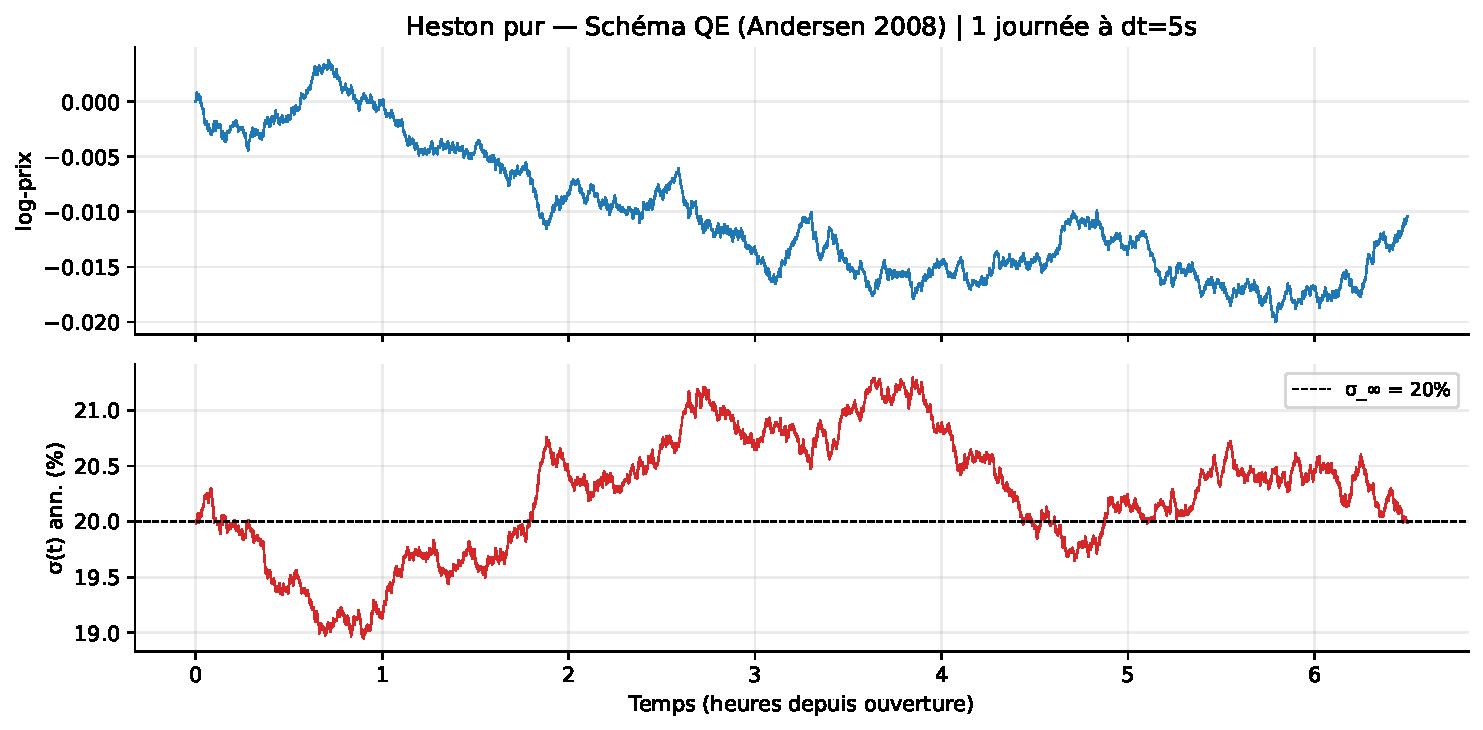
\includegraphics[width=0.85\textwidth]{../notebooks/figures/section2a_heston_path}
  \caption{Simulated Heston log-price path with stochastic volatility ($\kappa=2$, $\theta=0.04$, $\xi=0.5$, $\rho=-0.7$). The QE scheme guarantees $V_t \ge 0$.}
  \label{fig:heston_path}
\end{figure*}

\subsection{Merton model (compound Poisson jumps)}

The log-price follows the dynamics with compound Poisson jump process:
\begin{equation}\label{eq:merton}
  d\log S_t = (\mu - V_t/2 - \lambda\bar{k})\,dt + \sqrt{V_t}\,dW_t^S + J\,dN_t,
\end{equation}
where $N_t \sim \text{Poisson}(\lambda)$, $J \sim \mathcal{N}(\mu_J, \sigma_J^2)$,
and $\bar{k} = e^{\mu_J + \sigma_J^2/2} - 1$ corrects the drift so that $S_t$
is a martingale (Andersen-Benzoni-Lund 2002 parameterisation).

\paragraph{Grid parameterisation.}
Jump size is specified as a multiple of the local volatility:
\begin{align}
  \mu_J &= \texttt{jump\_size\_sigma} \times \sqrt{\theta} \times \sqrt{\dt},\nonumber\\
  \sigma_J &= 0.1 \times |\mu_J|.
\end{align}
For \texttt{jump\_size\_sigma} $= 5$ and $\dt t = 5\,\mathrm{s}$:
$\mu_J \approx 9.21 \times 10^{-4}$ (in log-price), a jump of size
$5\sigma\sqrt{\dt}$. Jump intensities per regime:
\begin{align}
  \lambda_\text{rare} &= 1\,500/\mathrm{year} \approx 0.64\text{ j/path},\nonumber\\
  \lambda_\text{moderate} &= 5\,000/\mathrm{year} \approx 2.12\text{ j/path}
\end{align}
for $n = 500$, $\dt t = 5\,\mathrm{s}$.

\begin{figure*}[t]
  \centering
  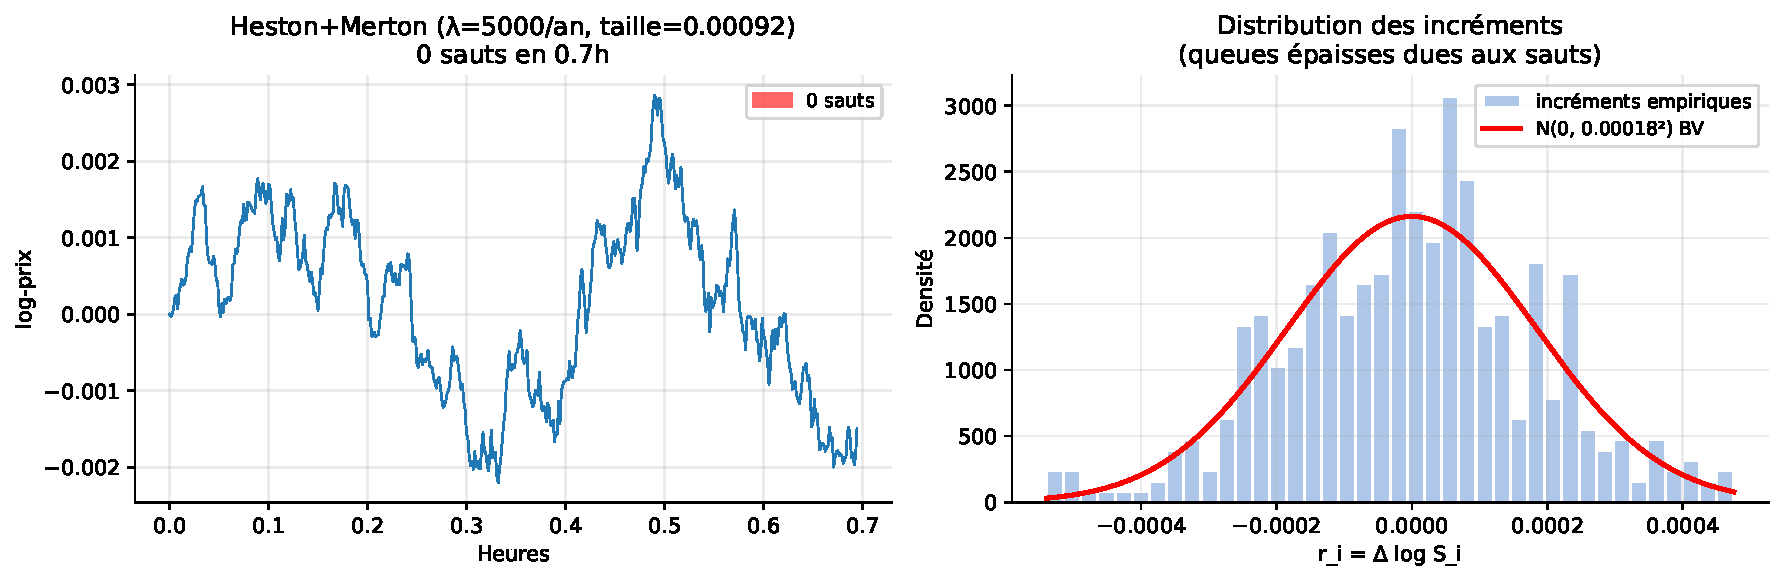
\includegraphics[width=0.85\textwidth]{../notebooks/figures/section2b_merton_hist}
  \caption{Distribution of Merton jump sizes under the three regimes (rare, moderate, hawkes\_dense). Jump sizes are specified as multiples of the local volatility $\hat{\sigma}_i\sqrt{\dt}$.}
  \label{fig:merton_hist}
\end{figure*}

\subsection{Self-exciting Hawkes process}

To model the temporal dependence of jumps, a discrete Hawkes process is used:
\begin{equation}\label{eq:hawkes}
  \lambda_{n+1} = \mu + (\lambda_n - \mu)\,e^{-\beta\dt t} + \alpha\,N_n,
\end{equation}
where $N_n \in \{0,1\}$ and $p_n = 1 - e^{-\lambda_n \dt}$.

\paragraph{Parameters.}
\begin{equation}
  \mu = 5\,000/\mathrm{year},\quad
  \alpha = 88\,000/\mathrm{year},\quad
  \beta = 0.03/\mathrm{s}.
\end{equation}
Branching ratio:
$m = \alpha / (\beta \times \mathrm{Seconds(per/year)}) = 88\,000 / (0.03 \times 5\,896\,800) \approx 0.497 < 1$.
Stationarity requires $m < 1$; an error is raised otherwise.

\paragraph{Validation.}
Over 30 seeds ($n = 200$, $\dt t = 5\,\mathrm{s}$): $3.8$ jumps/path vs.\
$1.3$ for \texttt{moderate} (ratio $\approx 3$).

\paragraph{Note on discretisation.}
At $\dt t = 300\,\mathrm{s}$, the approximation of the continuous Hawkes
process by this discrete scheme degrades. The process remains well-defined
($p_n \le 1$) but the low-frequency results for the \texttt{hawkes\_dense}
regime should be interpreted with care.

\subsection{Discretisation convention}

$\mathrm{Seconds(per/year)} = 252 \times 6.5 \times 3600 = 5\,896\,800$.
Returns $r_i$ are in natural log. $\dt$ is in years. The
\texttt{jump\_indices} provided by the simulator are indices into the
log-price array; the corresponding return index is $j - 1$.

\section{Spot volatility estimation}
\label{sec:estimators}

\subsection{Bipower variation (BNS 2004)}

\begin{definition}[BV]
\begin{equation}\label{eq:bv}
  \mathrm{BV}_n = \frac{\pi}{2} \cdot \frac{1}{n-1}
    \sum_{i=2}^{n} |r_{i-1}||r_i|.
\end{equation}
\end{definition}
Under pure diffusion, $\mathrm{BV}_n \to_P \int_0^T \sigma_t^2\,dt$.
Under jumps, BV is downward-biased: the products $|r_{i-1}||r_i|$ are close
to zero when one of the returns carries an isolated jump.

\subsection{MedRV and MinRV (ADS 2012)}

\begin{definition}[MedRV, ADS 2012 eq.~12]
\begin{align}\label{eq:medrv}
  \mathrm{MedRV}_n &= c_\mathrm{med} \cdot \tfrac{n}{n-2}
    \sum_{i=2}^{n-1} \mathrm{med}(|r_{i-1}|,|r_i|,|r_{i+1}|)^2,\nonumber\\
  c_\mathrm{med} &= \tfrac{\pi}{6-4\sqrt{3}+\pi} \approx 1.4191.
\end{align}
\end{definition}

\begin{definition}[MinRV, ADS 2012 eq.~13]
\begin{align}\label{eq:minrv}
  \mathrm{MinRV}_n &= c_\mathrm{min} \cdot \tfrac{n}{n-1}
    \sum_{i=2}^{n} \min(|r_{i-1}|,|r_i|)^2,\nonumber\\
  c_\mathrm{min} &= \tfrac{\pi}{\pi-2} \approx 2.7141.
\end{align}
\end{definition}

\subsection{Local spot volatility and causality condition}
\label{sec:spot}

The spot variance estimator computes $\hat{\sigma}^2(i)$ over a
window of $K$ returns \emph{strictly preceding} $i$:
\begin{equation}\label{eq:window}
  \hat{\sigma}^2(i) = \hat{V}(\log S[\max(0, i-K) : i+1],\; \dt t).
\end{equation}
The return $r_i$ is \textbf{never} included in the estimation window --- this
is the \emph{causality condition} required for $\hat{\sigma}_i$ to be
$\mathcal{F}_{i-1}$-measurable, ensuring $\E[E_i \mid \mathcal{F}_{i-1}] \le 1$.

The window is $K = 50$. The first $K$ hypotheses are excluded from
the test (incomplete window).


\paragraph{Classical test statistics.}
$L_i = r_i / (\hat{\sigma}_i\sqrt{\dt}) \approx \mathcal{N}(0,1)$ under
$H_{0,i}$ (Lee-Mykland), two-sided p-value $P_i = 2\Prob(|Z| > |L_i|)$.

\begin{figure*}[t]
  \centering
  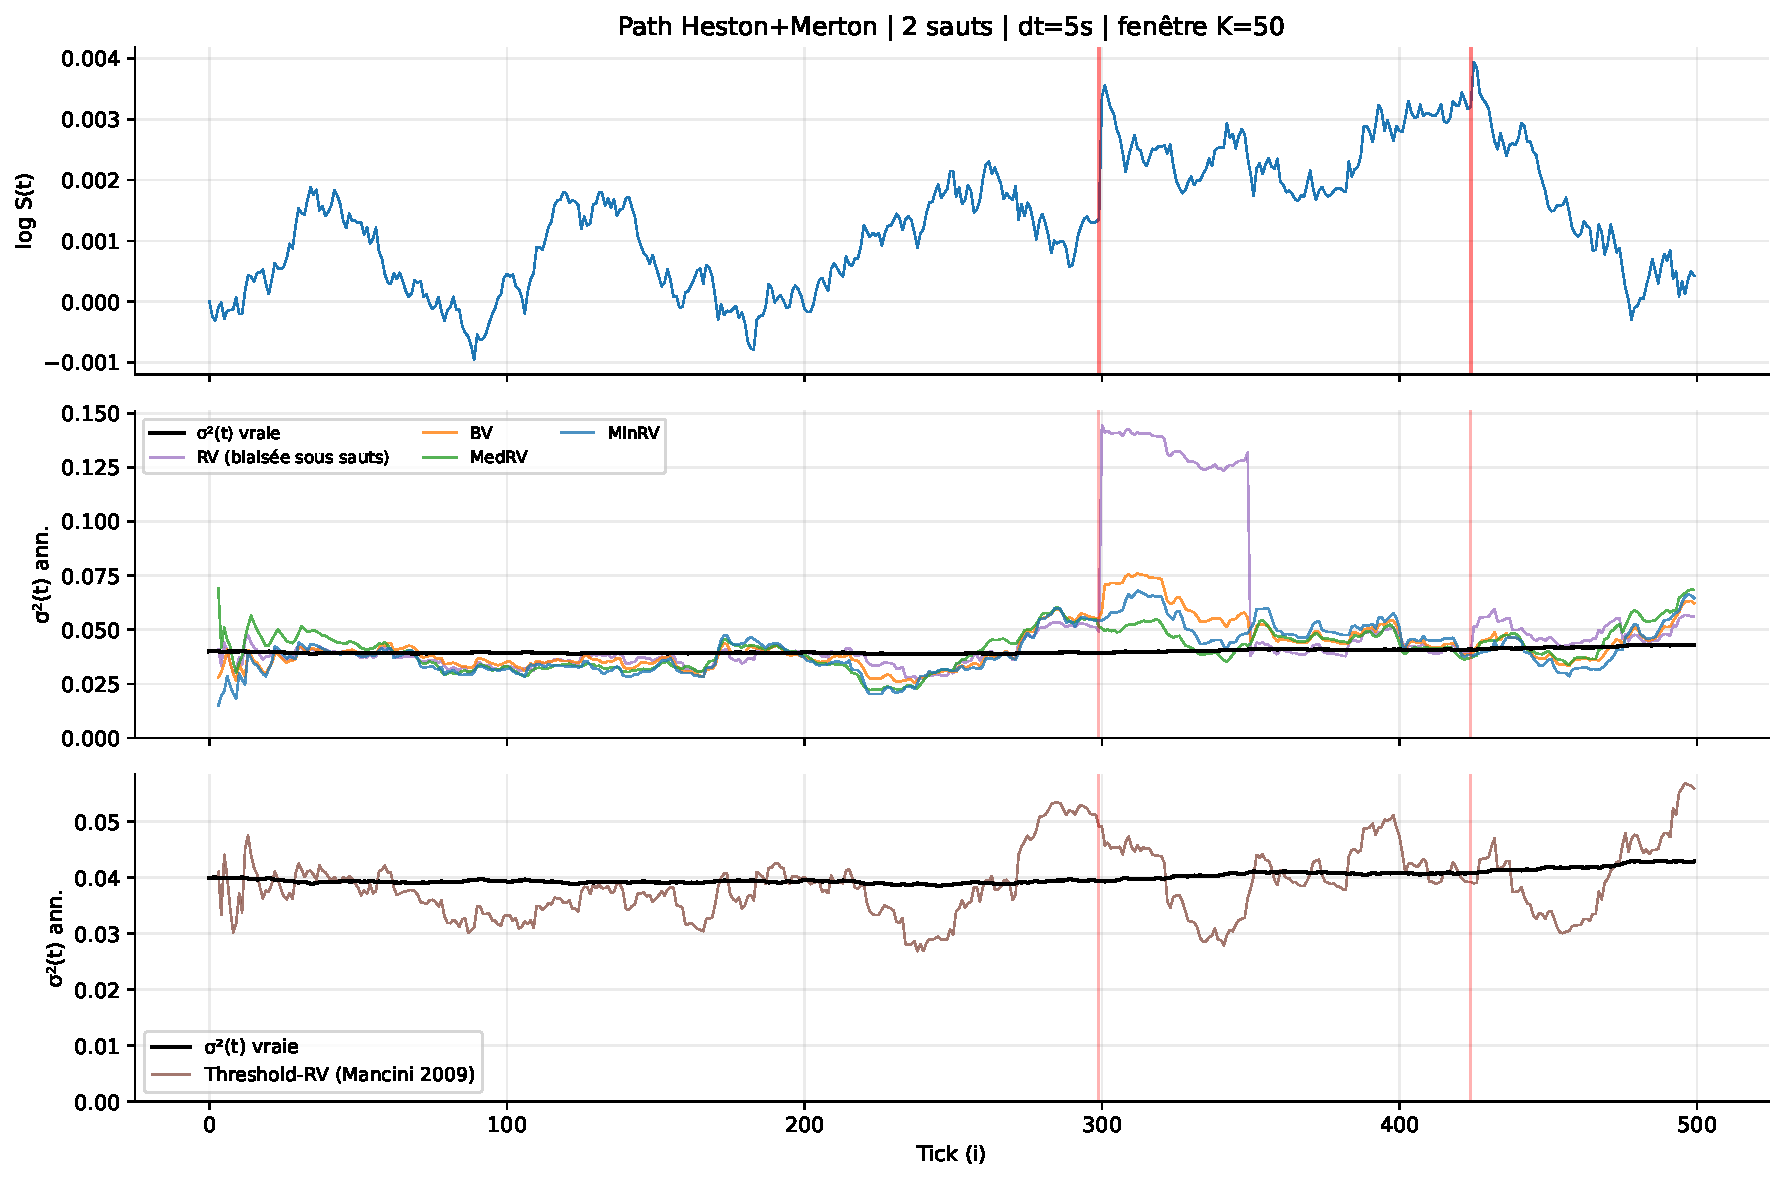
\includegraphics[width=0.85\textwidth]{../notebooks/figures/section3a_vol_estimators}
  \caption{Comparison of spot volatility estimators (BV, MedRV, MinRV) on a simulated Heston path with Merton jumps. MedRV is the most robust to jump contamination.}
  \label{fig:vol_estimators}
\end{figure*}


\section{E-value construction}
\label{sec:evalues}

\subsection{Local test formulation}

For each $H_{0,i}$:
\begin{align}
  H_{0,i} &: r_i \mid \mathcal{F}_{i-1} \sim \mathcal{N}(0,\; v), \quad v = \dt\,\hat{\sigma}_i^2, \\
  H_{1,i}(J) &: r_i \mid \mathcal{F}_{i-1} \sim \mathcal{N}(J,\; v)
\end{align}
for an unknown jump size $J$.

\subsection{Integrated likelihood ratio under a Gaussian prior}

The GROW construction chooses $\pi(J) = \mathcal{N}(0, \tau^2)$ and defines:
\begin{equation}\label{eq:evalue_integral}
  E_i = \int_{-\infty}^{+\infty}
    \frac{e^{Jr_i/v - J^2/(2v)}}{\sqrt{2\pi\tau^2}}\,
    e^{-J^2/(2\tau^2)}\, dJ.
\end{equation}

The derivation (Appendix~\ref{ann:grow}) gives the closed form:
\begin{equation}\label{eq:evalue}
  \boxed{E_i = \sqrt{\frac{v}{v + \tau^2}} \cdot
    \exp\!\left(\frac{r_i^2\,\tau^2}{2v(v + \tau^2)}\right)},
\end{equation}
with $v = \dt\,\hat{\sigma}_i^2$ and $\tau = 5\,\hat{\sigma}_i\sqrt{\dt}$.

\paragraph{Parameter \texttt{tau\_factor} $= 5$.}
$\tau = 5\,\hat{\sigma}_i\sqrt{\dt}$ places mass on jumps of size
$\pm 5\,\hat{\sigma}_i\sqrt{\dt}$, consistent with the grid regimes
($3\sigma$ and $5\sigma$).

\subsection{Validity: $\E[E_i \mid \mathcal{F}_{i-1}] = 1$ under $H_{0,i}$}

\begin{proposition}\label{prop:valid}
If $\hat{\sigma}_i$ is $\mathcal{F}_{i-1}$-measurable and $r_i \mid \mathcal{F}_{i-1} \sim \mathcal{N}(0, v)$ under $H_{0,i}$, then $\E[E_i \mid \mathcal{F}_{i-1}] = 1$.
\end{proposition}

\begin{proof}
$E_i = \int (dP_J/dP_0)(r_i)\,d\pi(J)$ is the marginal density under the
mixture divided by $P_0$. By Fubini:
$\E_{P_0}[E_i] = \int \E_{P_0}[dP_J/dP_0]\,d\pi(J) = \int 1\,d\pi(J) = 1$.
\end{proof}

The measurability condition is ensured by excluding the tested point from
the window (Section~\ref{sec:spot}).

\subsection{Empirical verification}

Four unit tests verify:
\begin{enumerate}
  \item \textbf{H0/H1 separation}: distribution of $E_i$ concentrated near 1
    under pure diffusion, shifted toward large values under a jump.
  \item \textbf{Monotone e-power}: $\E[\log E_i]$ strictly increasing in jump
    size (from $3\sigma$ to $7\sigma$).
  \item \textbf{Dominance over p-to-e}: e-power of the GROW construction
    exceeds that of the $\kappa = 0.5$ calibrator.
  \item \textbf{Validity}: $\E[E_i] \le 1 + 3\,\mathrm{SE}$ under $H_0$,
    $M = 10\,000$.
\end{enumerate}

\begin{figure*}[t]
  \centering
  \begin{subfigure}[b]{0.48\textwidth}
    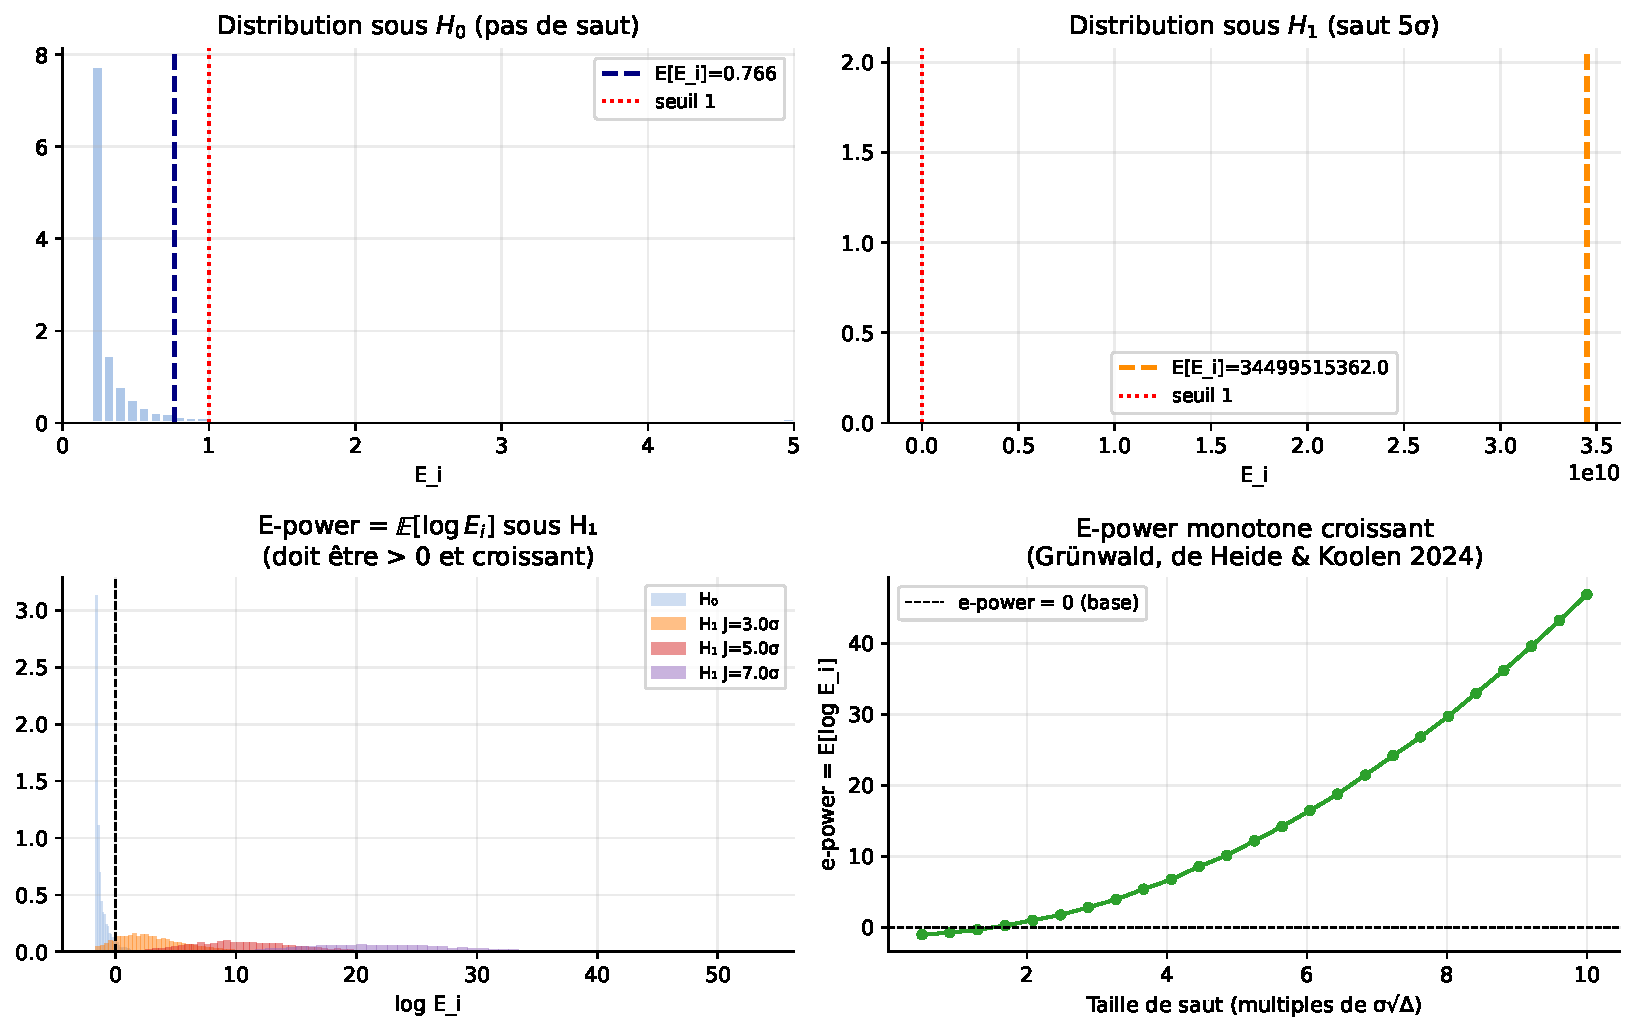
\includegraphics[width=\textwidth]{../notebooks/figures/section4a_evalue_distributions}
    \caption{Distribution of $E_i$ under $H_0$ and $H_1$.}
    \label{fig:evalue_dist}
  \end{subfigure}
  \hfill
  \begin{subfigure}[b]{0.48\textwidth}
    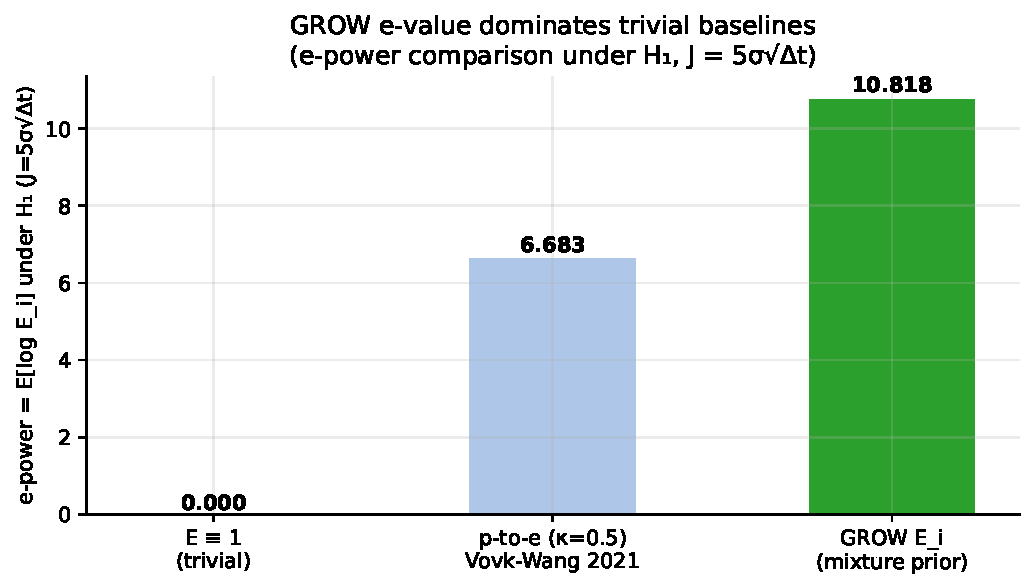
\includegraphics[width=\textwidth]{../notebooks/figures/section4b_epower_comparison}
    \caption{E-power: GROW vs.\ Vovk-Wang calibrator ($\kappa=0.5$).}
    \label{fig:epower_cmp}
  \end{subfigure}
  \caption{Empirical validation of the GROW e-value construction. Left: under $H_0$ the distribution is concentrated near 1; under $H_1$ it is shifted to large values. Right: the GROW construction dominates the baseline calibrator in e-power across jump sizes.}
  \label{fig:evalues_validation}
\end{figure*}



\section{Online FDR control procedures}
\label{sec:fdr}

This section presents the seven procedures benchmarked in
Section~\ref{sec:results}. The exposition follows the offline to online
progression set up in Section~\ref{sec:metrics}: e-BH is offline, e-LOND,
e-LORD, e-SAFFRON, and stopped e-BH are online. Proofs of FDR control rely
on the e-value framework of Section~\ref{sec:pe}.

\subsection{e-BH (Wang \& Ramdas 2022)}
\label{sec:ebh}

The e-BH procedure is the e-value analogue of Benjamini-Hochberg. Before
stating it, we need the notion of \emph{compound e-variables}, which extends
e-variables to sets of indices.

\begin{definition}[Compound e-variables]
Let $H_1, \ldots, H_K$ be null hypotheses and $E_1, \ldots, E_K$ non-negative
random variables. They are \emph{compound e-variables} for
$(H_1, \ldots, H_K)$ if
\[
  \E\!\left[\sum_{k \in N} E_k\right] \leq |N|
\]
for every configuration of true nulls $N \subseteq [K]$. They are
\emph{tight} if equality holds for some $N$.
\end{definition}

A collection of $K$ e-variables is automatically a collection of compound
e-variables, but the converse is false in general.

\begin{definition}[e-BH, Wang \& Ramdas 2022]
Let $e_1, \ldots, e_K$ be realised compound e-values and let $e_{[k]}$ denote
the $k$-th order statistic from the largest to the smallest. The e-BH
procedure at level $\alpha \in (0,1)$ rejects the hypotheses corresponding to
the largest $k^*$ e-values, where
\[
  k^* := \max\!\left\{k : \frac{k\,e_{[k]}}{K} \geq \frac{1}{\alpha}\right\}
\]
($k^* := 0$ if the set is empty).
\end{definition}

If $k^* = 0$, no hypothesis is rejected. The
complexity is $O(K \log K)$ for sorting.

\begin{theorem}[Wang \& Ramdas 2022]\label{thm:ebh}
For arbitrary dependence among the e-values, the e-BH procedure at level
$\alpha$ satisfies
\[
  \FDR \leq \alpha \cdot \frac{|N|}{K} \leq \alpha.
\]
\end{theorem}

The proof factors through a generic property called \emph{self-consistency},
which characterises a broad class of FDR-controlling procedures.

\begin{definition}[Self-consistency]
An e-testing procedure $D$ is \emph{self-consistent at level $\alpha$} if for
every $k \in D$:
\[
  e_k \geq \frac{K}{\alpha\,R_D}.
\]
\end{definition}

\begin{proposition}\label{prop:sc}
The e-BH procedure is self-consistent. Moreover, any self-consistent
e-testing procedure at level $\alpha$ has $\FDR \leq \alpha K_0 / K$ for
arbitrary configurations of e-values, where $K_0 = |N|$.
\end{proposition}

\begin{proof}{\small
By self-consistency, for every $k \in D$:
$\ind_{\{k \in D\}}/R_D \leq \alpha E_k/K$.
Summing over $N$: $F_D/(R_D\vee 1) \leq \sum_{k\in N}\alpha E_k/K$.
Taking expectations and using $\E[E_k]\leq 1$:
$\FDR \leq \alpha K_0/K$.
Self-consistency of e-BH follows by construction: $e_k \geq e_{[R_D]} \geq K/(\alpha R_D)$.
}\end{proof}

Theorem~\ref{thm:ebh} follows by Proposition~\ref{prop:sc} applied to e-BH.


\subsection{e-LOND (Xu \& Ramdas 2024)}
\label{sec:elond}

The online setting requires a different machinery: e-values arrive in a
stream $(E_t)_{t \ge 1}$ and decisions must be made on the fly. We work with
the natural filtration $\mathcal{F}_t = \sigma(E_1, \ldots, E_t)$,
$\mathcal{F}_0$ trivial.

\begin{definition}[e-process]
An \emph{e-process} is a non-negative adapted sequence $(E_t)_{t \geq 0}$
such that for every stopping time $\tau$ w.r.t.\ $(\mathcal{F}_t)$,
$\E[E_\tau] \leq 1$.
\end{definition}

Since FDR is by definition the expectation of a proportion whose numerator
and denominator may both be unbounded as $t \to \infty$, we work with the
running quantity $\FDR(t)$.

\begin{definition}[e-LOND, Xu \& Ramdas 2024]
At step $t \geq 1$, set
\begin{align}\label{eq:elond}
  \alpha_t &= \alpha \cdot \gamma_t \cdot (R_{t-1} + 1),\nonumber\\
  \gamma_t &= C_\mathrm{JM} \cdot
    \frac{\log\max(t,2)}{t \cdot \exp\!\sqrt{\log\max(t,2)}},
\end{align}
where $R_{t-1}$ is the number of rejections before time $t$ and
$(\gamma_t)_{t \geq 1}$ is a user-chosen non-increasing non-negative sequence
satisfying $\sum_{t \geq 1} \gamma_t \leq 1$ (the choice above is the
Javanmard-Montanari sequence). Reject $H_t$ iff $E_t \geq 1/\alpha_t$.
\end{definition}

\paragraph{Constant $C_\mathrm{JM} = 0.15708906$.}
Verified by truncated summation up to $t = 10^6$:
$\sum_{t=1}^{10^6} \gamma_t \approx 1.00000$.

\paragraph{Interpretation.}
The budget $\alpha \sum_t \gamma_t \leq \alpha$ is distributed over time. The
factor $(R_{t-1}+1)$ raises the rejection threshold after each rejection
(wealth accumulation). The decay $\gamma_t \sim \log(t)/(t\,e^{\sqrt{\log t}})$
ensures validity for infinite streams.

\begin{theorem}[Xu \& Ramdas 2024]
e-LOND controls $\FDR \le \alpha$ under arbitrary dependence.
\end{theorem}

\subsection{e-LORD (e-GAI framework, Zhang et al.\ 2025)}
\label{sec:elord}

e-LORD takes a more flexible route via an \emph{oracle FDP estimator}. The
decision rule is again $\delta_t = \ind_{\{E_t \geq 1/\alpha_t\}}$, but
$\alpha_t$ is now built from an estimator that adapts to the rejection
history.

Define the (unobservable) \emph{oracle FDP}:
\[
  FDP^*(t) = \sum_{j \in H_0(t)} \frac{\alpha_j}{R_{j-1} + 1}.
\]
It is called \emph{oracle} because the summation runs over true nulls
$H_0(t)$, which are unknown. The corresponding (observable) e-LORD estimator
sums over all hypotheses:
\[
  \widehat{FDP}_{\text{e-LORD}}(t) = \sum_{j=1}^{t} \frac{\alpha_j}{R_{j-1} + 1}.
\]

\begin{proposition}\label{prop:oracle-fdr}
If $\E[FDP^*(t)] \leq \alpha$ for all $t \geq 1$, then $\FDR(t) \leq \alpha$
for all $t \geq 1$.
\end{proposition}

\begin{proof}{\small
By Markov $\delta_j\leq\alpha_j E_j$ and $R_t\vee 1\geq R_{j-1}+1$, so
$\FDR(t)\leq \E[\sum_{j\in H_0}\alpha_j E_j/(R_{j-1}+1)]
\leq \E[\sum_{j\in H_0}\alpha_j/(R_{j-1}+1)] = \E[FDP^*(t)]\leq\alpha$,
using $\E[E_j\mid\mathcal{F}_{j-1}]\leq 1$.
}\end{proof}

Since $H_0(t) \subseteq \{1, \ldots, t\}$ and all terms $\alpha_j/(R_{j-1}+1)
\geq 0$,
\[
  FDP^*(t) \leq \widehat{FDP}_{\text{e-LORD}}(t)
\]
almost surely, giving the FDR guarantee.

\paragraph{Risk-aversion allocation rule.}
The testing levels $\alpha_t$ are set via the \emph{Risk Aversion Investing}
(RAI) rule of Zhang et al.\ (2025):
\begin{align}\label{eq:alphat}
  \alpha_t &= \omega_t \cdot rw_t \cdot (R_{t-1} + 1),\nonumber\\
  rw_t &= \alpha - \sum_{j=1}^{t-1} \frac{\alpha_j}{R_{j-1}+1},
\end{align}
where $rw_t$ is the \emph{remaining wealth} and $(\omega_t)_{t \in
\mathbb{N}} \in (0,1)$ governs the fraction of remaining wealth allocated to
the current test. Initial wealth $rw_1 = \alpha$, $\alpha_1 = \alpha
\omega_1$. The sequence $\omega_t$ updates as
\begin{equation}\label{eq:omegat}
  \omega_{t+1} = \omega_t + \omega_1\,\phi^{t-R_t}(1-\delta_t) - \omega_1\,\psi^{R_t}\delta_t,
\end{equation}
with user-chosen parameters $\phi, \psi \in [0, 0.5]$ ensuring $\omega_t \in
(0,1)$.

\begin{algorithm*}
\caption{e-LORD}
\label{alg:elord}
\begin{algorithmic}[1]
\Require Initial wealth $rw_1 = \alpha$, sequence $(\omega_t)$, parameters $\phi, \psi$
\State $R_0 \leftarrow 0$
\For{$t = 1, 2, \ldots$}
    \State $\alpha_t \leftarrow \omega_t \cdot rw_t \cdot (R_{t-1} + 1)$
    \State Observe e-value $e_t$
    \If{$e_t \geq 1/\alpha_t$}
        \State Reject $H_t$; $\delta_t \leftarrow 1$
    \Else
        \State Accept $H_t$; $\delta_t \leftarrow 0$
    \EndIf
    \State $R_t \leftarrow R_{t-1} + \delta_t$
    \State $rw_{t+1} \leftarrow rw_t - \alpha_t/(R_{t-1}+1)$
    \State Update $\omega_{t+1}$ via \eqref{eq:omegat}
\EndFor
\end{algorithmic}
\end{algorithm*}

\begin{remark}[e-LOND as a special case]
Setting $\gamma_t = \omega_t \prod_{j=1}^{t-1}(1 - \omega_j)$ in e-LOND
recovers $\alpha_t^{\text{e-LOND}} = \alpha_t$ from \eqref{eq:alphat}. e-LOND
is therefore a particular instantiation of the RAI framework with a static
$\gamma_t$ schedule.
\end{remark}


\paragraph{Alpha-death.}
With $\omega_1 = 0.1$ over $n = 500$, e-LORD and e-SAFFRON exhaust their
wealth by $t \approx 50$ (power $\approx 0.002$). The canonical value is
$\omega_1 = O(1/T)$ (Zhang et al.\ 2025): for $n = 500$, take
$\omega_1 \leq 0.01$.

\subsection{e-SAFFRON (e-GAI framework, Zhang et al.\ 2025)}
\label{sec:esaffron}

e-SAFFRON is the \emph{adaptive} variant of e-LORD. It introduces a
predictable sequence $(\lambda_t)_{t \geq 1} \subset (0,1)$ estimating the
proportion of true nulls and \emph{discards} candidate nulls whose e-values
are too small, reallocating $\alpha$-wealth toward more informative
hypotheses.

The corresponding FDP estimator is
\[
  \widehat{FDP}_{\text{e-SAFFRON}}(t)
    = \sum_{j=1}^{t} \frac{\alpha_j}{R_{j-1} + 1}
      \cdot \frac{\ind_{\{e_j < 1/\lambda_j\}}}{1 - \lambda_j}.
\]
The intuition: when $e_j \geq 1/\lambda_j$, the hypothesis is a candidate
alternative and is not charged to the FDP estimate; otherwise it contributes
with inverse weight $(1 - \lambda_j)^{-1}$.

\begin{theorem}
Let $(E_t)_{t \geq 1}$ be an e-process and $(\lambda_t)_{t \geq 1}$ a
predictable sequence in $(0,1)$. Then for every $t \geq 1$:
\[
  \E[\widehat{FDP}_{\text{e-SAFFRON}}(t)] \geq \E[FDP^*(t)].
\]
\end{theorem}

\begin{proof}{\small
Since $\lambda_j$ is $\mathcal{F}_{j-1}$-measurable, Markov gives
$\Prob(E_j < 1/\lambda_j\mid\mathcal{F}_{j-1})\geq 1-\lambda_j$ under $H_{0,j}$.
Restricting the sum to $j\in H_0(t)$ and applying this bound:
$\E[\widehat{FDP}_{\text{e-SAFFRON}}(t)]
\geq \sum_{j\in H_0(t)}\E[\alpha_j/(R_{j-1}+1)]
= \E[FDP^*(t)]$.
}\end{proof}

Combining with Proposition~\ref{prop:oracle-fdr}, e-SAFFRON controls
$\FDR \leq \alpha$ at every $t$.

\paragraph{Remaining-wealth rule.}
The testing levels use a modified wealth
\[
  rw_t^{\text{e-SAFFRON}} = \alpha(1 - \lambda)
    - \sum_{j=1}^{t-1} \frac{\alpha_j\,\ind_{\{e_j < 1/\lambda_j\}}}{R_{j-1}+1},
\]
and $\alpha_t = \omega_t \cdot rw_t^{\text{e-SAFFRON}} \cdot (R_{t-1}+1)$,
with $\omega_t$ updated by~\eqref{eq:omegat}. The rejection rule remains
$\delta_t = \ind_{\{e_t \geq 1/\alpha_t\}}$.


\begin{algorithm*}
\caption{e-SAFFRON}
\label{alg:esaffron}
\begin{algorithmic}[1]
\Require Initial wealth $rw_1 = \alpha(1 - \lambda)$, predictable sequence $(\lambda_t)$, parameters $\phi, \psi$
\State $R_0 \leftarrow 0$
\For{$t = 1, 2, \ldots$}
    \State $\alpha_t \leftarrow \omega_t \cdot rw_t^{\text{e-SAFFRON}} \cdot (R_{t-1}+1)$
    \State Observe $e_t$
    \If{$e_t \geq 1/\alpha_t$}
        \State Reject $H_t$; $\delta_t \leftarrow 1$
    \Else
        \State Accept $H_t$; $\delta_t \leftarrow 0$
    \EndIf
    \State $R_t \leftarrow R_{t-1} + \delta_t$
    \State $rw_{t+1}^{\text{e-SAFFRON}} \leftarrow rw_t^{\text{e-SAFFRON}} - \alpha_t \ind_{\{e_t < 1/\lambda_t\}}/(R_{t-1}+1)$
    \State Update $\omega_{t+1}$ via \eqref{eq:omegat}
\EndFor
\end{algorithmic}
\end{algorithm*}

Setting $\lambda = 0$ recovers e-LORD: e-SAFFRON is therefore the adaptive
counterpart of e-LORD.

\subsection{Stopped e-BH (Wang, Dandapanthula \& Ramdas 2025)}
\label{sec:stopped}

The offline e-BH procedure (Section~\ref{sec:ebh}) requires all e-values to
be available at once. In sequential settings, data arrive over time and one
may want to stop the experiment at a data-dependent time while still
controlling FDR. The stopped e-BH procedure addresses this.

The key subtlety is the notion of filtration. Suppose $G$ null hypotheses
$H_0^1, \ldots, H_0^G$ are tested simultaneously, each with its own
\emph{local} filtration $(\mathcal{F}_n^g)_{n \geq 0}$ generated from the
data specific to hypothesis $g$. The \emph{global} filtration is
$\mathcal{F}_n = \sigma(\mathcal{F}_n^g : g \in [G])$. Let $\mathcal{T}$
denote the set of stopping times w.r.t.\ $(\mathcal{F}_n)$.

\begin{definition}[Global e-process]
A non-negative adapted process $(M_n^g)_{n \geq 1}$ is a \emph{global
e-process} for $\mathcal{P}^g$ on $(\mathcal{F}_n)$ if at any stopping time
$\tau \in \mathcal{T}$, $M_\tau^g$ is an e-value for $\mathcal{P}^g$:
$\sup_{P \in \mathcal{P}^g} \E^P[M_\tau^g] \leq 1$.
\end{definition}

A process that is an e-process only w.r.t.\ its local filtration
$(\mathcal{F}_n^g)$ is a \emph{local} e-process. The distinction is crucial:
stopping a local e-process at a global stopping time $\tau \in \mathcal{T}$
does \emph{not} in general yield a valid e-value, which would invalidate the
FDR guarantee.

\begin{definition}[Stopped FDR control]
An adapted sequence of random sets $(R_n)$ with $R_n \subseteq [G]$
satisfies \emph{level-$\alpha$ stopped FDR control} if
\[
  \sup_{P \in \mathcal{M},\, \tau \in \mathcal{T}} FDR_\tau \leq \alpha,
\]
where $FDR_\tau = \E^P[FDP_\tau]$ and $FDP_\tau = FD_\tau / (R_\tau \vee 1)$.
\end{definition}

\begin{definition}[Stopped e-BH]
Run e-BH at each time step on the current values of the e-processes:
$R_n = eBH_\alpha(M_n^g : g \in [G])$.
\end{definition}

\begin{theorem}[Stopped e-BH, Wang et al.\ 2025]\label{thm:stopped}
Let $(M_n^g)_{n \geq 1}$, $g \in [G]$, be global e-processes for
$(\mathcal{P}^g : g \in [G])$. Then $(R_n) = \{eBH_\alpha(M_n^g : g \in [G])\}$
satisfies level-$\alpha$ stopped FDR control.
\end{theorem}

\begin{proof}
Fix $\tau \in \mathcal{T}$ and $P \in \mathcal{M}$. Each $(M_n^g)$ being a
global e-process, the stopped values $(M_\tau^g : g \in [G])$ are valid
e-values. Theorem~\ref{thm:ebh} (FDR control of offline e-BH under arbitrary
dependence) applied to these stopped e-values gives $FDR_\tau \leq \alpha$
for the set $eBH_\alpha(M_\tau^g : g \in [G])$. Since this holds for any
$\tau$ and $P$, stopped FDR control follows.
\end{proof}

This reduces the problem to verifying that locally constructed e-processes
are in fact global. Wang et al.\ (2025) identify a Markovian causal
condition under which this holds.

\begin{definition}[Markovian assumption, Wang et al.\ 2025, Assumption 3.1]
Consider observations $Z_n = (X_n, Y_n)$ where $X_n \in \mathcal{X}$ is a
covariate and $Y_n = (Y_n^1, \ldots, Y_n^G) \in \mathcal{Y}^1 \times \cdots
\times \mathcal{Y}^G$ a response vector. The Markovian assumption is
\[
  Y_n \perp (X_1,\ldots,X_{n-1};Y_1,\ldots,Y_{n-1}) \mid X_n
  \quad \forall\, n \geq 2.
\]
Given the current covariate $X_n$, $Y_n$ is independent of the past, with
arbitrary cross-component dependence in $Y_n$ allowed.
\end{definition}

Under this assumption, any e-process built multiplicatively from stepwise
e-values computed within a single hypothesis is globally valid (Wang et
al.\ 2025, Theorem 3.3), covering likelihood-ratio and universal-inference
e-processes.

\paragraph{Application to jump detection.}
In our setting, the Markovian assumption is satisfied by the causal window
of Section~\ref{sec:spot}: $\hat{\sigma}_i$ is $\mathcal{F}_{i-1}$-measurable
(does not look at $r_i$), so $E_i$ is a global e-value. Complexity is
$O(t \log t)$ per step.

\subsection{Baselines BH-LM and BH-BNS}

\paragraph{BH-LM.}
BH-LM computes $L_i = r_i / (\hat{\sigma}_i\sqrt{\dt})$, the two-sided
p-value $P_i = 2\Prob(|Z| > |L_i|)$, then applies BH. Decisions are made
per hypothesis.

\paragraph{BH-BNS.}
BH-BNS applies a global BNS ratio test and duplicates its result across all
hypotheses: if the global test rejects, all returns are flagged as jumps;
otherwise none. This matches the BS 2016 usage (BNS as a day-level filter).

\subsection{Synthetic comparison}

\begin{table*}[t]
\centering
\caption{Summary: guarantees, assumptions, complexity.}
\label{tab:procs_detail}
\begin{tabular}{lcccc}
\toprule
Procedure & Guarantee & Dependence & Key parameter & Complexity \\
\midrule
e-BH & $\FDR \le \alpha$ & Arbitrary & --- & $O(n\log n)$ \\
e-LOND & $\FDR \le \alpha$ & Arbitrary & $C_\mathrm{JM}$ & $O(1)$/step \\
e-LORD & $\FDR \le \alpha$ & Arbitrary & $\omega_1, \phi, \psi$ & $O(1)$/step \\
e-SAFFRON & $\FDR \le \alpha$ & Arbitrary & $\omega_1, \lambda$ & $O(1)$/step \\
Stopped e-BH & Anytime $\FDR \le \alpha$ & Markov / causal & --- & $O(t\log t)$/step \\
BH-LM & $\FDR \le \alpha$ & PRDS & $K_\mathrm{win}$ & $O(n\log n)$ \\
BH-BNS & $\FDR \le \alpha$ & PRDS & --- & $O(n)$ \\
\bottomrule
\end{tabular}
\end{table*}


\section{Software architecture and pipeline}
\label{sec:pipeline}

\subsection{Five-layer structure}

\begin{center}
\texttt{simulate} $\to$ \texttt{estimators} $\to$ \texttt{evalues} $\to$
\texttt{fdr} $\to$ \texttt{pipeline}
\end{center}


\subsection{Metrics}

\begin{align*}
  \FDP &= \tfrac{|\mathcal{R}\cap\mathcal{H}_0|}{\max(|\mathcal{R}|,1)}, &
  \text{Power} &= \tfrac{|\mathcal{R}\cap\mathcal{H}_1|}{\max(|\mathcal{H}_1|,1)},\\
  \text{F1} &= \tfrac{2\,\text{Prec}\cdot\text{Rec}}{\text{Prec}+\text{Rec}},\\
  \text{Delay} &= \tfrac{\sum_{i\in\mathcal{R}\cap\mathcal{H}_1}(t_i-t_{i,\text{true}})}{|\mathcal{R}\cap\mathcal{H}_1|}.
\end{align*}

\paragraph{Reading the metrics.}
Each hypothesis $H_{0,i}$ targets a single tick $i$; the simulator provides
the ground truth $\mathcal{H}_1$ (true jump indices). Three path-level
quantities complement FDR and power:
\begin{itemize}[noitemsep]
  \item \textbf{Precision} $= |\mathcal{R}\cap\mathcal{H}_1|/\max(|\mathcal{R}|,1)$:
    fraction of declared jumps that are genuine --- the per-path analogue of
    $1 - \mathrm{FDP}$.
  \item \textbf{Recall} $= |\mathcal{R}\cap\mathcal{H}_1|/\max(|\mathcal{H}_1|,1)$:
    fraction of true jumps that are detected --- the per-path analogue of
    power.
  \item \textbf{F1} $= 2\,\mathrm{Precision}\cdot\mathrm{Recall}/(\mathrm{Precision}+\mathrm{Recall})$:
    harmonic mean of the two; the natural scalar summary when precision and
    recall trade off against each other.
  \item \textbf{Delay}: average number of ticks between the true jump index
    and the rejection index, over correctly detected jumps. Since each
    hypothesis $H_{0,i}$ is decided at tick $i$ (one-to-one correspondence),
    the delay is zero whenever the procedure rejects the exact tick of the
    jump and positive only if a neighbouring tick is rejected instead.
    Offline procedures (e-BH, BH-LM) are always zero-delay; online procedures
    may differ depending on the volatility window.
\end{itemize}

\section{Empirical results}
\label{sec:results}

\subsection{Protocol}

\textbf{Source}: \texttt{results/grid\_medium.parquet} 

\begin{table*}[t]
\centering
\caption{Parameters of the \texttt{grid\_medium}.}
\label{tab:grid}
\begin{tabular}{ll}
\toprule
Parameter & Value \\
\midrule
$n_\text{steps}$ & 500 \\
Frequencies ($\Delta t$, s) & [5, 60, 300] \\
Jump regimes & [rare, moderate, hawkes\_dense] \\
Jump sizes ($\sigma$) & [3, 5] \\
$\alpha$ & [0.05, 0.10] \\
$\omega_1$ (e-LORD/e-SAFFRON) & [0.1, 0.5] \\
$M$ replications & 100 \\
Estimator & MedRV \\
Algorithms & 7 (see Table~\ref{tab:procs}) \\
Total tasks & 32\,400 \\
Duration & $\approx 7\,\mathrm{min}$ \\
\bottomrule
\end{tabular}
\end{table*}

\paragraph{FDR violation convention.}
For $\alpha = 0.05$, $M = 100$:
$\mathrm{SE} = \sqrt{\alpha(1-\alpha)/M} = \sqrt{0.05 \times 0.95/100} \approx 0.0218$.
Violation threshold: $\alpha + 2\,\mathrm{SE} \approx 0.094$.

\subsection{Result 1: BH's FDR violation at high frequency}

\begin{table*}[t]
\centering
\caption{Empirical FDR per algorithm $\times$ frequency ($\alpha = 0.05$, all regimes, $M = 100$, $n = 500$). Source: \texttt{grid\_medium.parquet}.}
\label{tab:fdr_freq}
\begin{tabular}{lcccl}
\toprule
Algorithm & $\Delta t = 5\,\mathrm{s}$ & $\Delta t = 60\,\mathrm{s}$ & $\Delta t = 300\,\mathrm{s}$ & Violates? \\
\midrule
BH-BNS & \textbf{0.096} & 0.022 & 0.002 & \textcolor{red}{\textbf{Yes}} \\
BH-LM & \textbf{0.096} & 0.022 & 0.002 & \textcolor{red}{\textbf{Yes}} \\
Stopped e-BH & 0.016 & 0.005 & 0.000 & \textcolor{teal}{No} \\
e-BH & 0.010 & 0.003 & 0.000 & \textcolor{teal}{No} \\
e-LOND & 0.001 & 0.000 & 0.000 & \textcolor{teal}{No} \\
e-LORD ($\omega_1 = 0.1$) & 0.000 & 0.000 & 0.000 & \textcolor{teal}{No} (alpha-death) \\
e-SAFFRON ($\omega_1 = 0.1$) & 0.000 & 0.000 & 0.000 & \textcolor{teal}{No} (alpha-death) \\
\midrule
\multicolumn{4}{l}{\textit{Violation threshold}: $0.094 = \alpha + 2\,\mathrm{SE}$} & \\
\bottomrule
\end{tabular}
\end{table*}

\paragraph{Interpretation.}
The violation operates through two distinct channels. For BH-BNS, the BNS
statistic is built on bipower variation, which is downward-biased whenever two
consecutive returns both carry a jump --- an event that becomes frequent under
the moderate and hawkes\_dense regimes at $5\,\mathrm{s}$. The resulting
under-estimation of integrated variance inflates the BNS ratio and triggers
spurious detections. For BH-LM, the mechanism is more subtle: although MedRV
is markedly more jump-robust than BV, the normalised statistics
$L_i = r_i / (\hat{\sigma}_i\sqrt{\dt})$ are computed over overlapping windows
of $K = 50$ returns. At $5\,\mathrm{s}$, these windows share a large fraction
of their returns, and under dense jump clustering the dependence structure of
the $L_i$ violates the PRDS condition that BH requires to guarantee
$\FDR \le \alpha$. In both cases the violation is structural: it does not
disappear with larger sample size, only with a stronger theoretical guarantee
(e.g.\ arbitrary-dependence e-value procedures).

Figure~\ref{fig:fdr_freq} illustrates the evolution of empirical FDR by
frequency for $\alpha = 0.05$ and $\alpha = 0.10$.

\begin{figure*}[t]
  \centering
  \begin{subfigure}[b]{0.48\textwidth}
    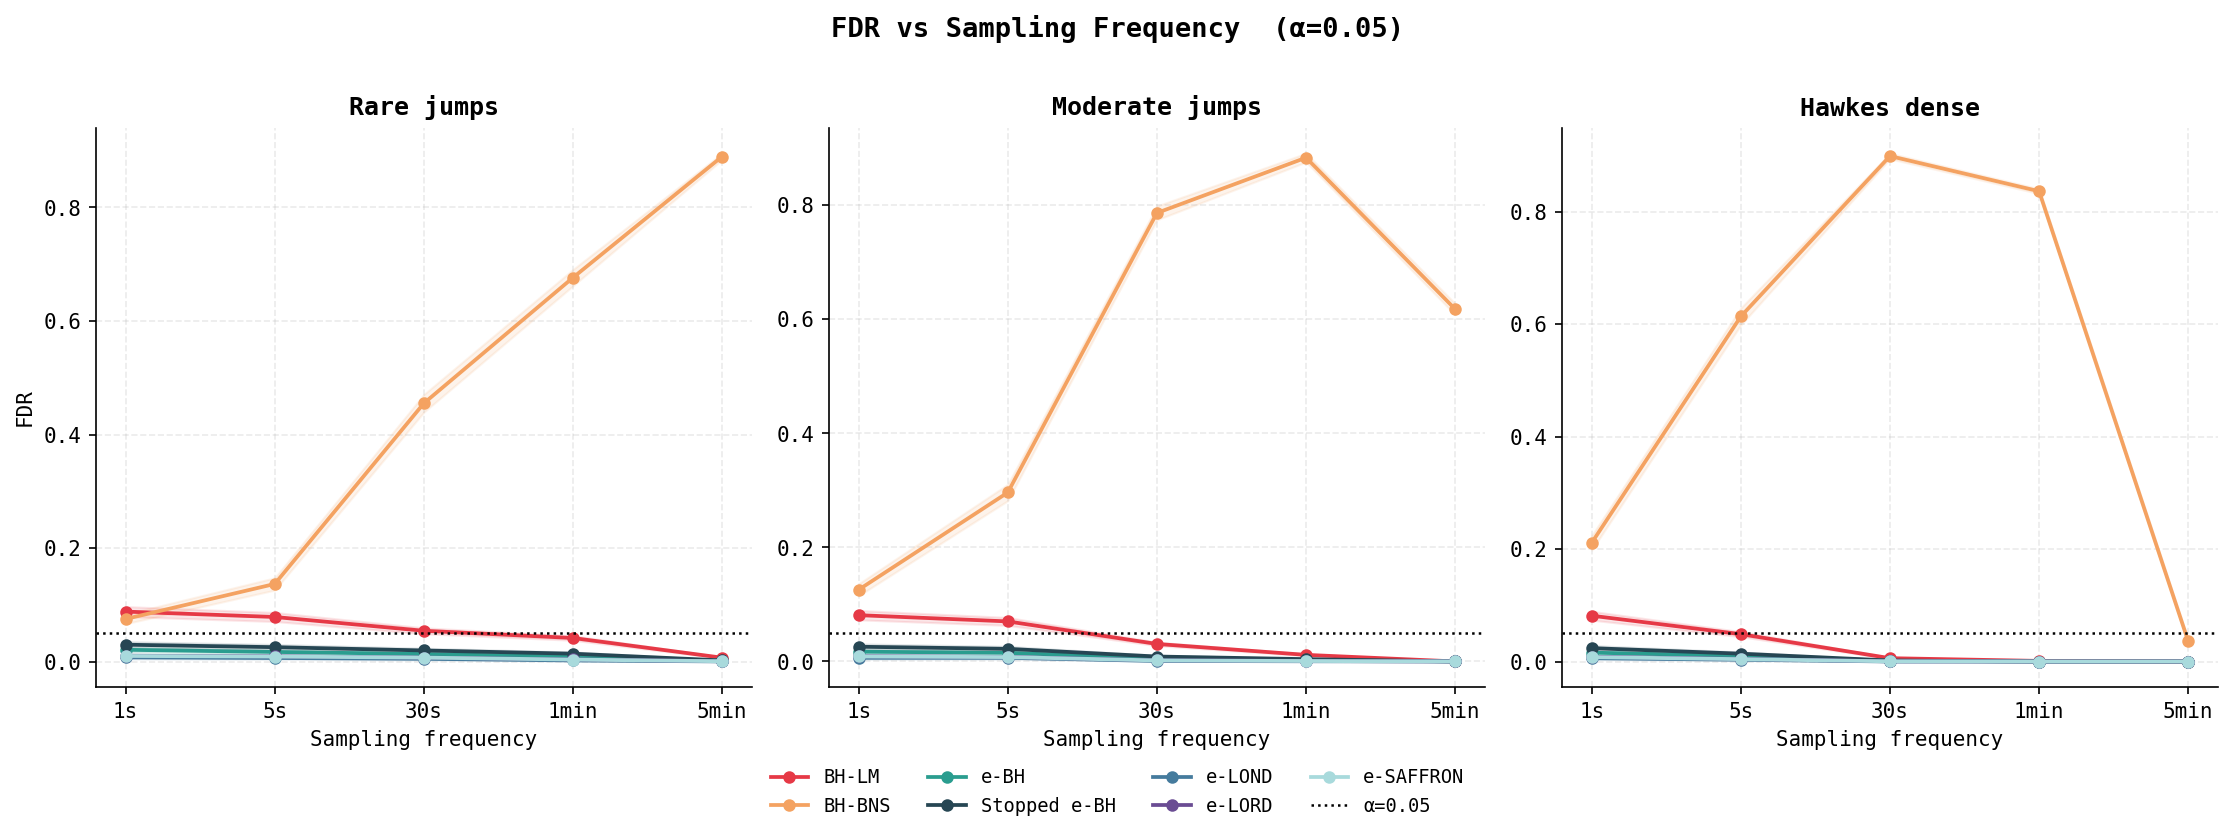
\includegraphics[width=\textwidth]{../results/figures/fig1_fdr_vs_freq_alpha5.png}
    \caption{$\alpha = 0.05$}
  \end{subfigure}
  \hfill
  \begin{subfigure}[b]{0.48\textwidth}
    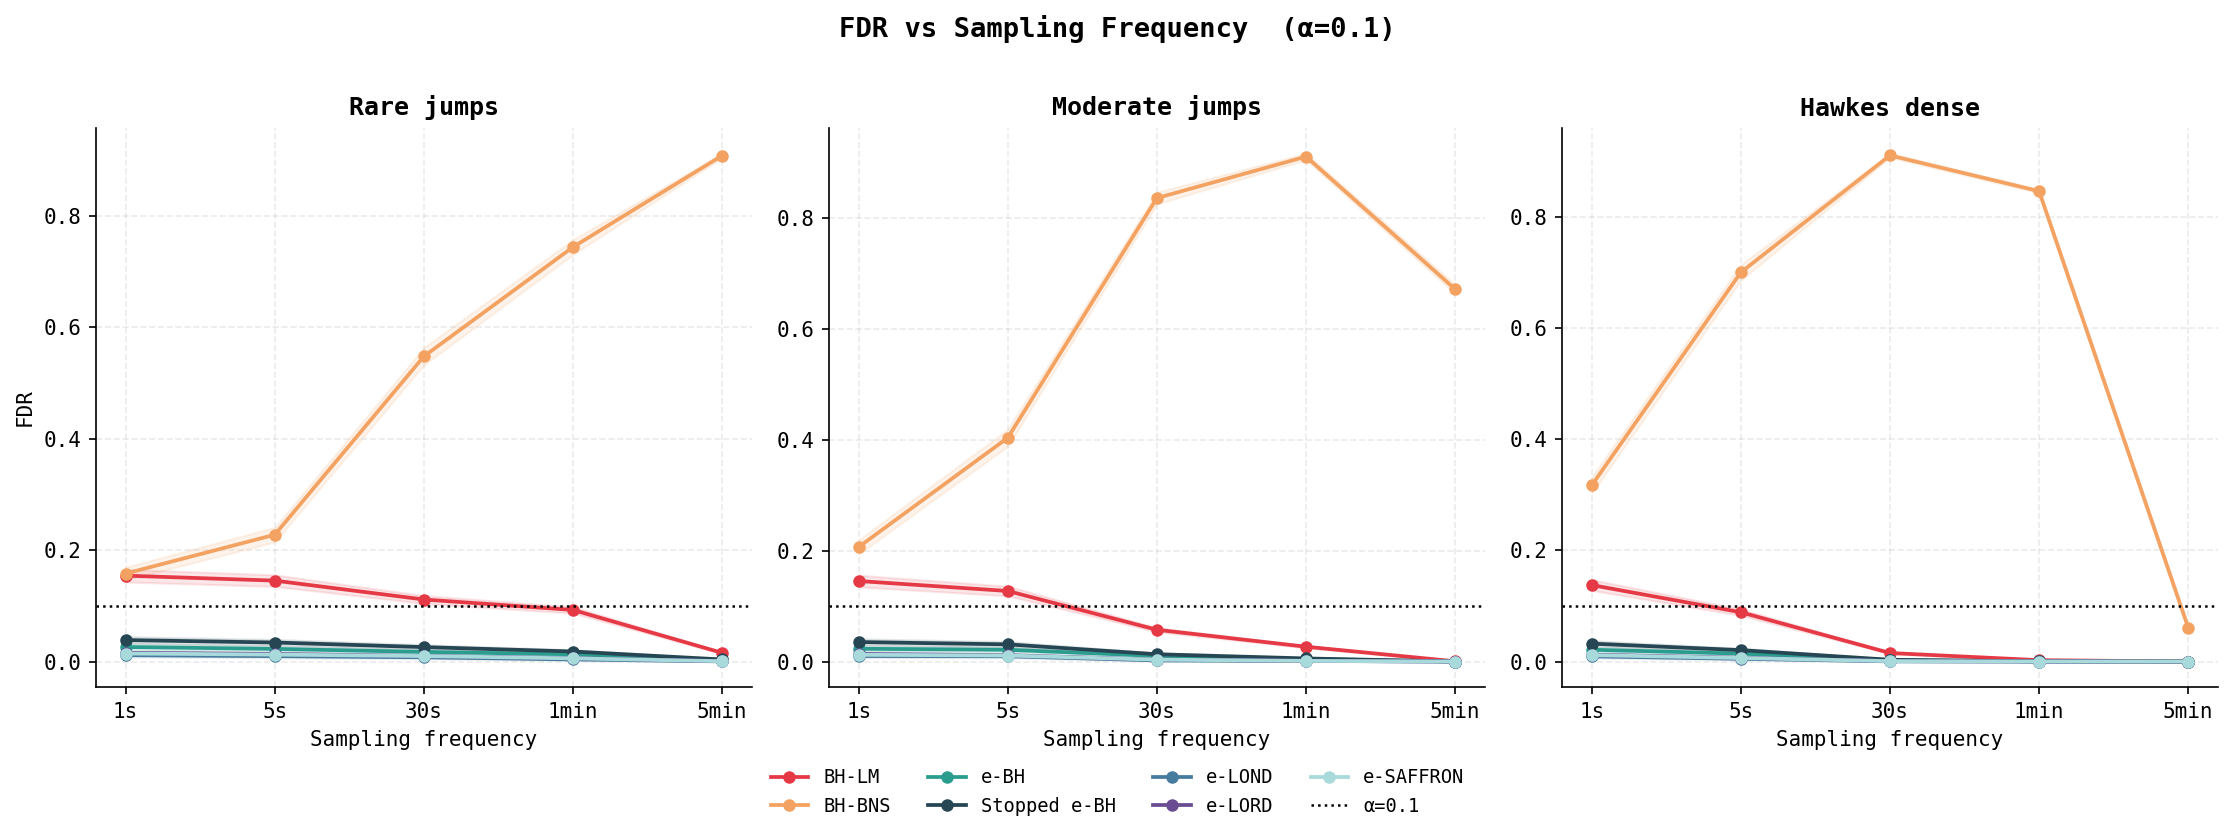
\includegraphics[width=\textwidth]{../results/figures/fig1_fdr_vs_freq_alpha10.png}
    \caption{$\alpha = 0.10$}
  \end{subfigure}
  \caption{Empirical FDR vs.\ sampling frequency, by algorithm and regime
  (\texttt{grid\_medium}, $M=100$). The dashed line marks the nominal level
  $\alpha$. BH-LM and BH-BNS exceed $\alpha$ at $5\,\mathrm{s}$ in all
  regimes.}
  \label{fig:fdr_freq}
\end{figure*}

\subsection{Result 2: e-value-based FDR control at all frequencies}

E-value-based procedures control the FDR at all tested frequencies
(stopped e-BH $\le 0.016$, e-BH $\le 0.010$, e-LOND $\le 0.001$) under the
three jump regimes, demonstrating robustness to the temporal dependence of
Hawkes jumps.


\subsection{Result 3: power-safety trade-off}

\begin{table*}[t]
\centering
\caption{Power per algorithm $\times$ frequency ($\alpha = 0.05$, all regimes). Source: \texttt{grid\_medium.parquet}.}
\label{tab:power_freq}
\begin{tabular}{lccc}
\toprule
Algorithm & $\Delta t = 5\,\mathrm{s}$ & $\Delta t = 60\,\mathrm{s}$ & $\Delta t = 300\,\mathrm{s}$ \\
\midrule
BH-BNS / BH-LM & 0.441 & 0.358 & 0.157 \\
Stopped e-BH & 0.349 & 0.258 & 0.028 \\
e-BH & 0.326 & 0.252 & 0.027 \\
e-LOND & 0.235 & 0.168 & 0.013 \\
e-LORD ($\omega_1 = 0.1$) & 0.002 & 0.001 & 0.000 \\
e-SAFFRON ($\omega_1 = 0.1$) & 0.002 & 0.001 & 0.000 \\
\bottomrule
\end{tabular}
\end{table*}

Among procedures that actually control the FDR, \textbf{stopped e-BH} is
the best compromise (power $0.349$ vs.\ e-BH $0.326$, e-LOND $0.235$). The
loss relative to BH (uncontrolled) is $9$--$21$ pp at $5\,\mathrm{s}$.

\begin{figure*}[t]
  \centering
  \begin{subfigure}[b]{0.48\textwidth}
    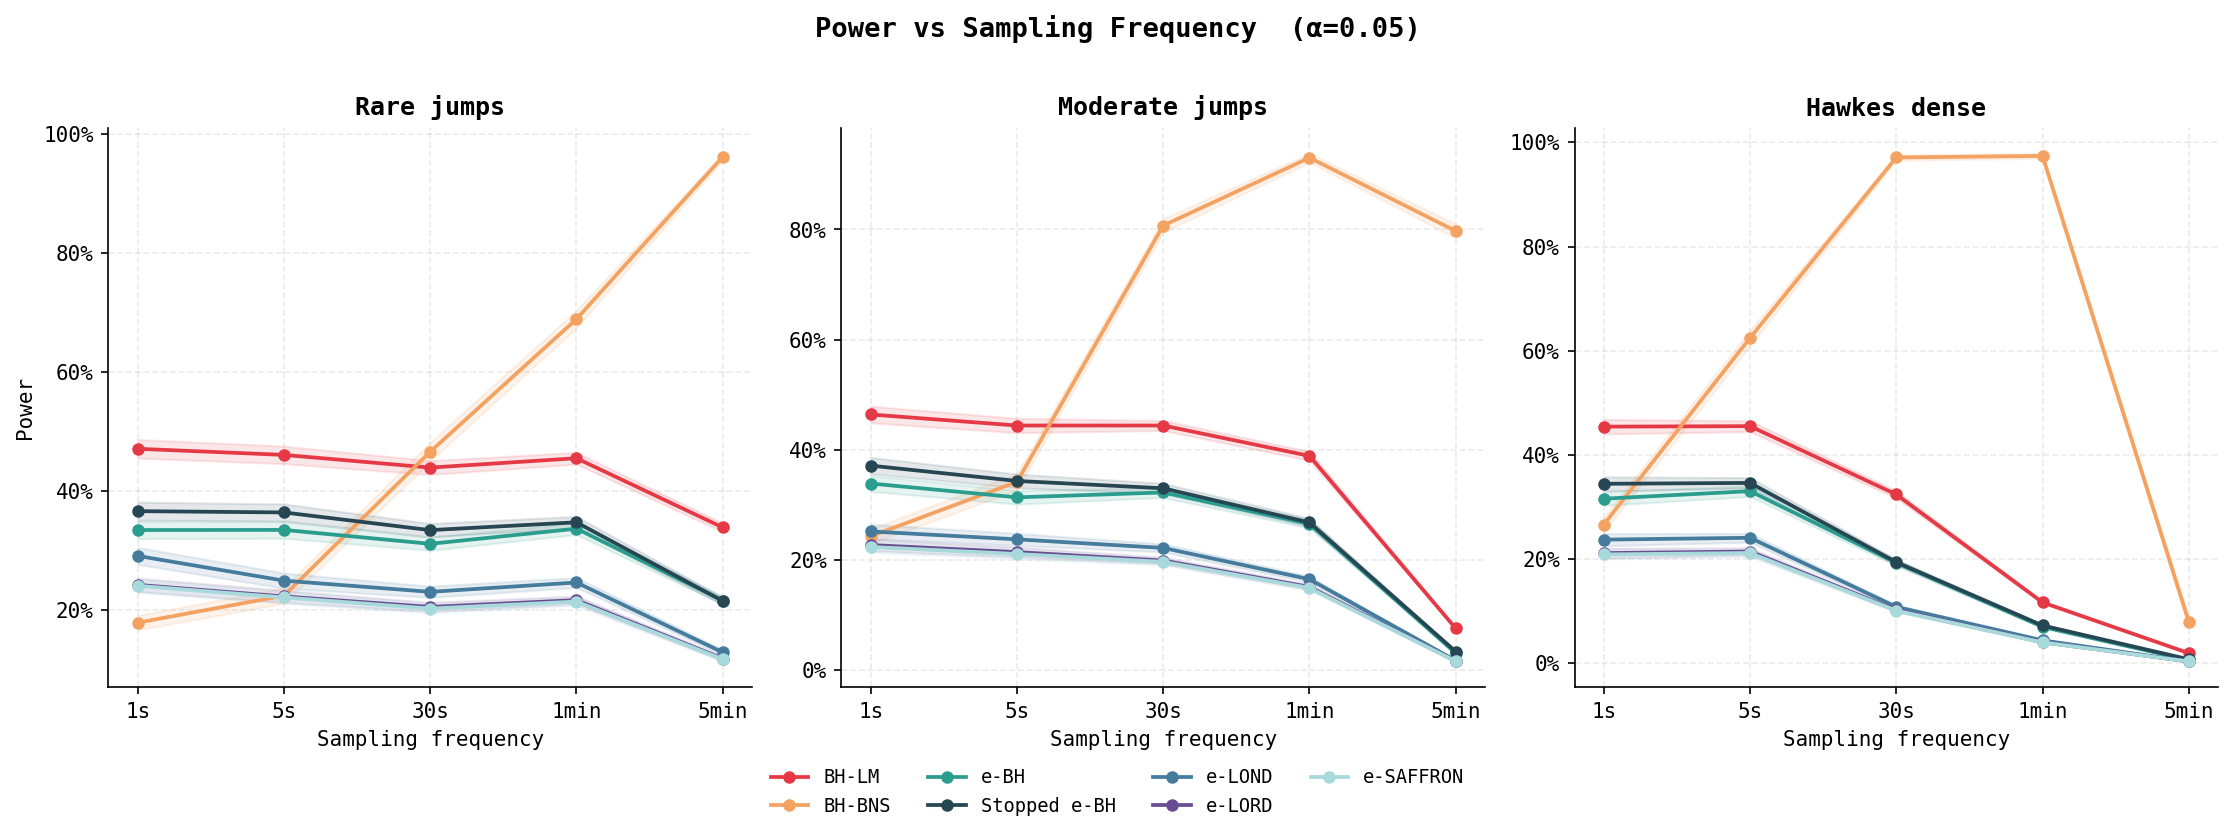
\includegraphics[width=\textwidth]{../results/figures/fig2_power_vs_freq_alpha5.png}
    \caption{$\alpha = 0.05$}
  \end{subfigure}
  \hfill
  \begin{subfigure}[b]{0.48\textwidth}
    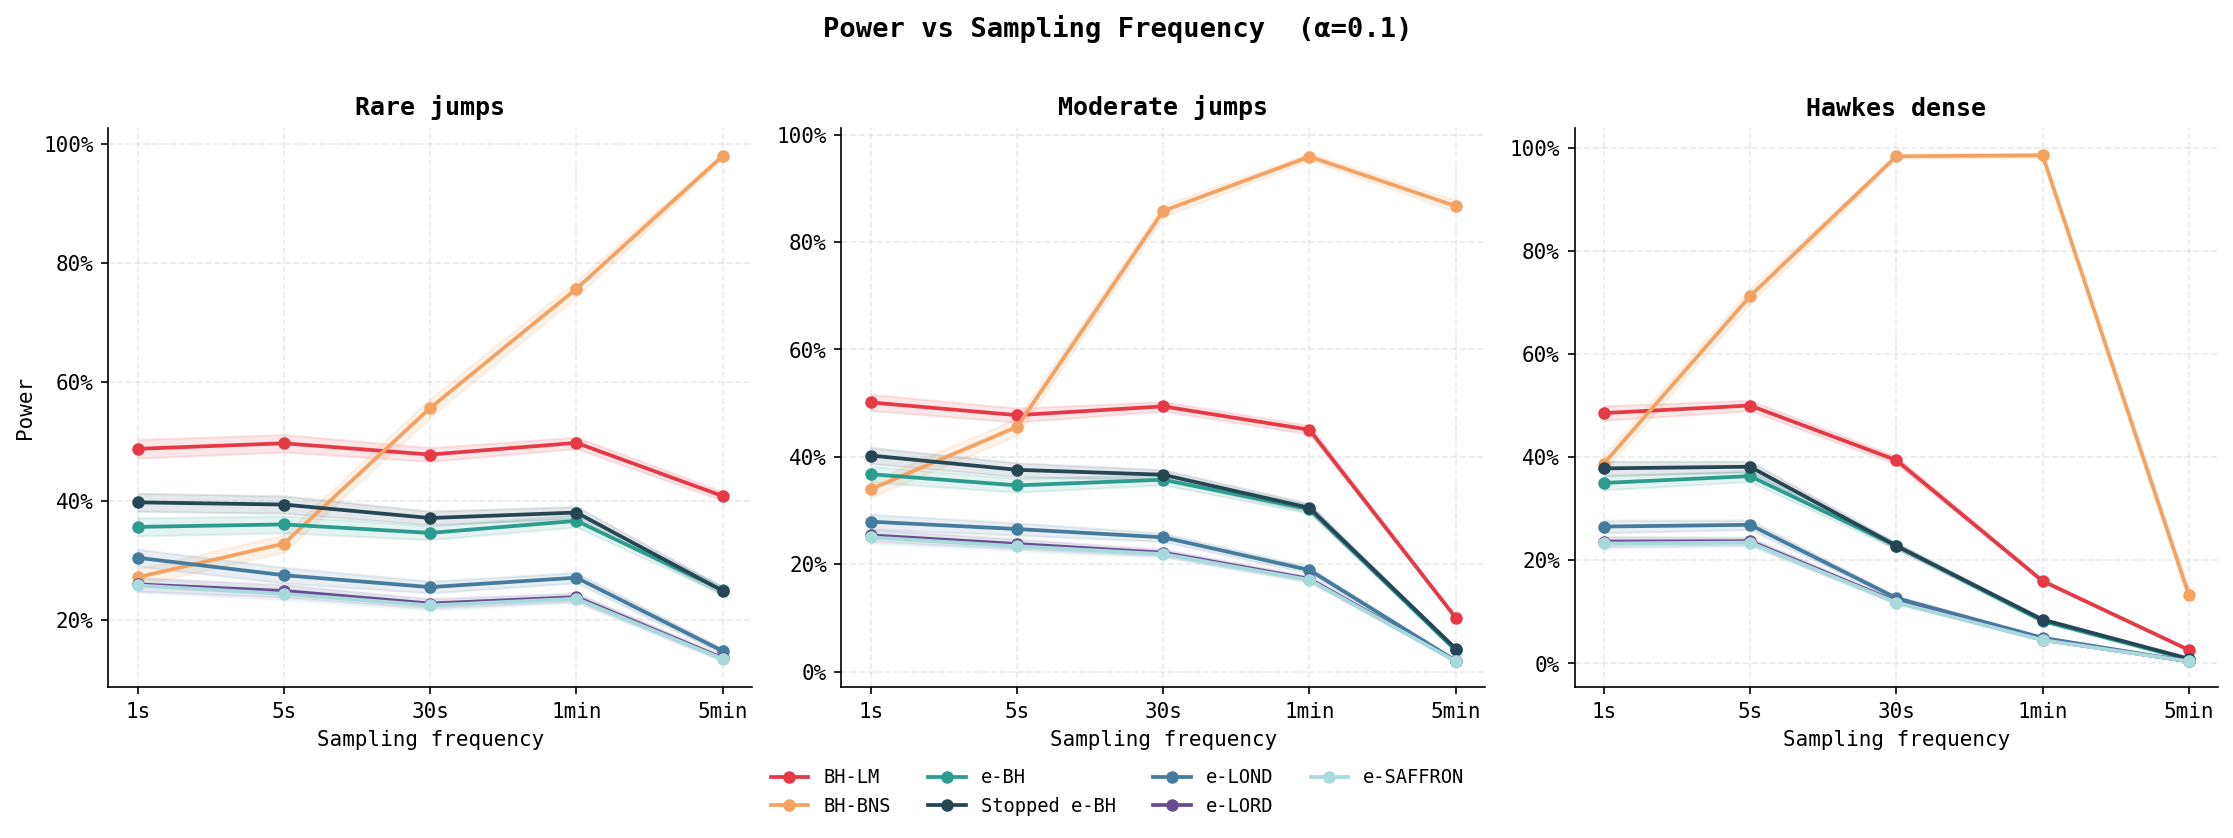
\includegraphics[width=\textwidth]{../results/figures/fig2_power_vs_freq_alpha10.png}
    \caption{$\alpha = 0.10$}
  \end{subfigure}
  \caption{Power vs.\ sampling frequency by algorithm and regime. Stopped
  e-BH dominates e-BH and e-LOND at all frequencies among valid procedures.
  e-LORD/e-SAFFRON with $\omega_1 = 0.1$: alpha-death at $5\,\mathrm{s}$.}
  \label{fig:power_freq}
\end{figure*}

\subsection{Result 4: FDR-power frontier}

\begin{figure*}[t]
  \centering
  \begin{subfigure}[b]{0.48\textwidth}
    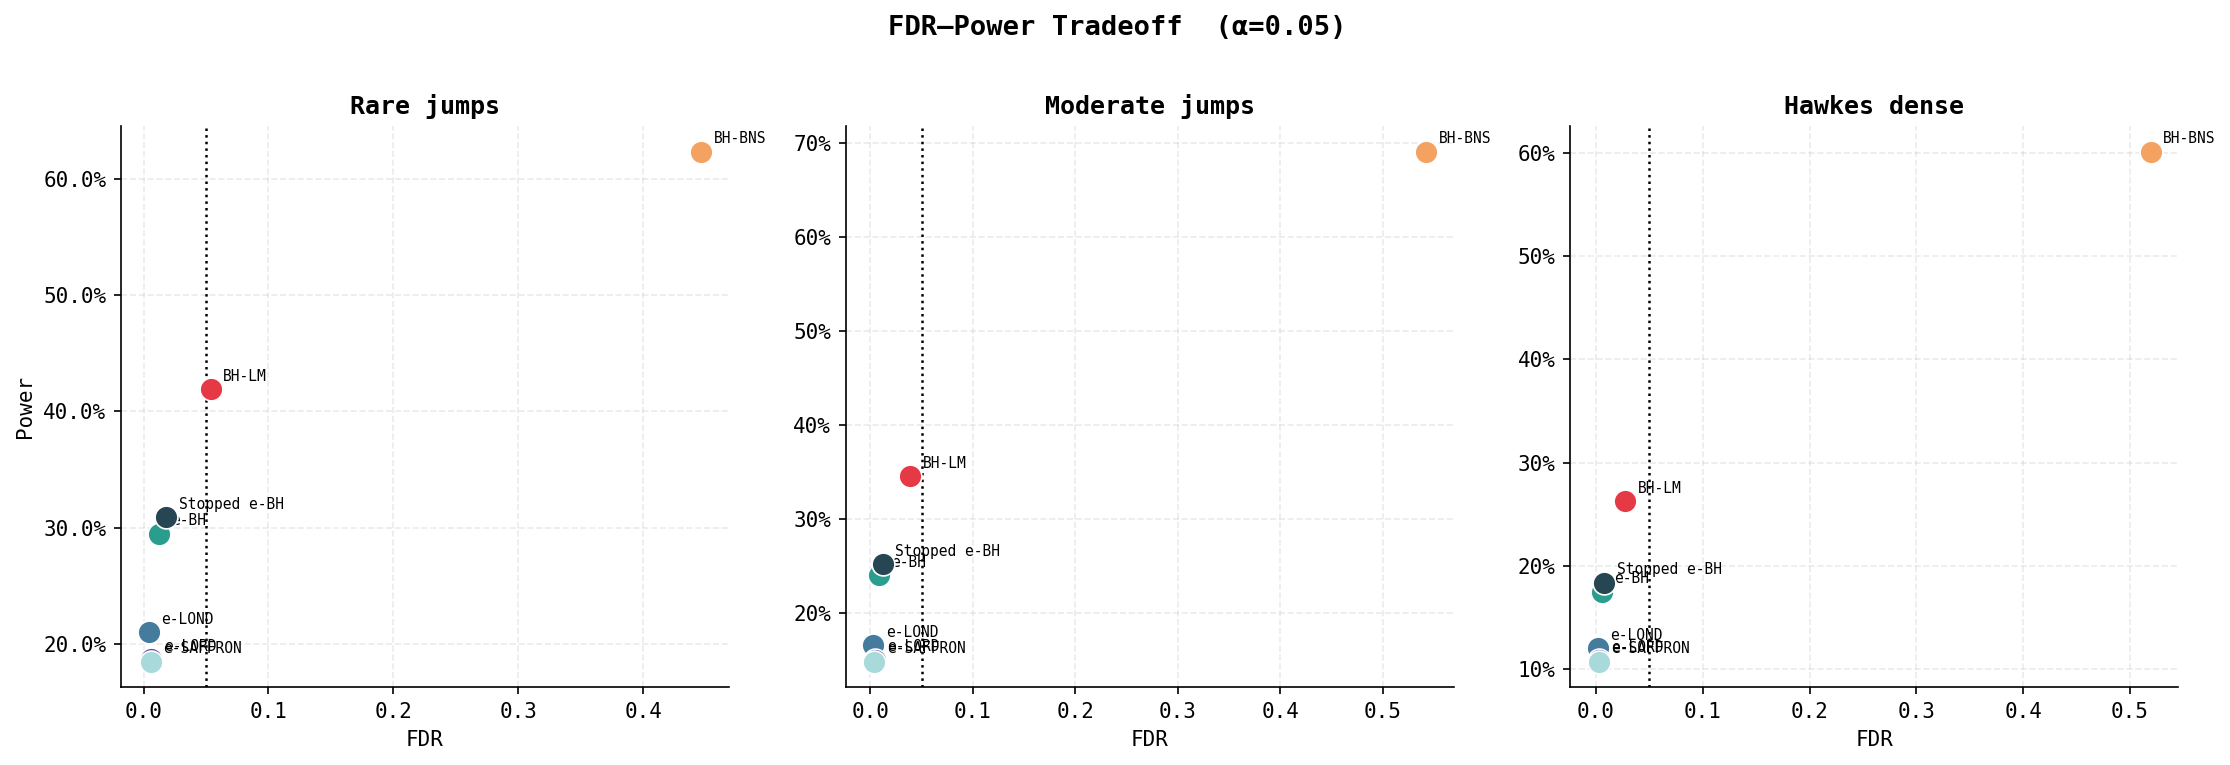
\includegraphics[width=\textwidth]{../results/figures/fig3_tradeoff_alpha5.png}
    \caption{$\alpha = 0.05$}
  \end{subfigure}
  \hfill
  \begin{subfigure}[b]{0.48\textwidth}
    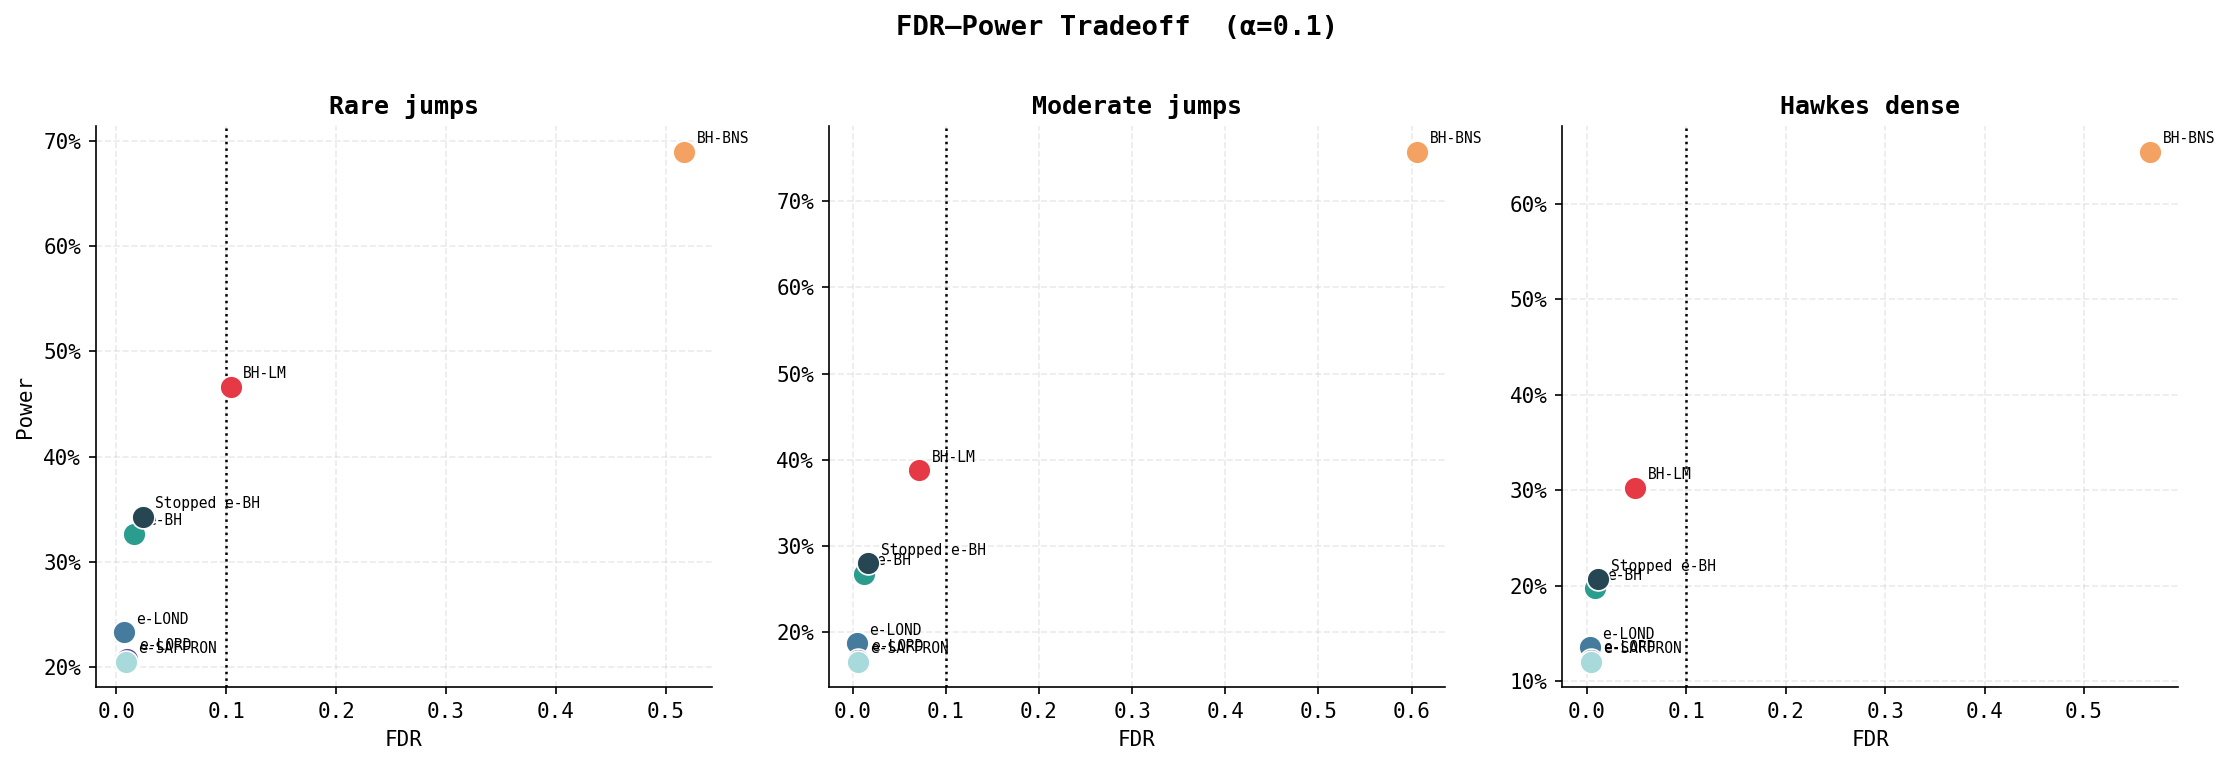
\includegraphics[width=\textwidth]{../results/figures/fig3_tradeoff_alpha10.png}
    \caption{$\alpha = 0.10$}
  \end{subfigure}
  \caption{Scatter of empirical FDR vs.\ power, by algorithm and regime.
  The dashed vertical line marks the nominal $\alpha$. BH procedures sit
  to the right (uncontrolled FDR, high power); e-value procedures sit to
  the left (controlled FDR, lower power).}
  \label{fig:tradeoff}
\end{figure*}

\subsection{Result 5: Hawkes intensity and jump clustering}

\begin{figure*}[t]
  \centering
  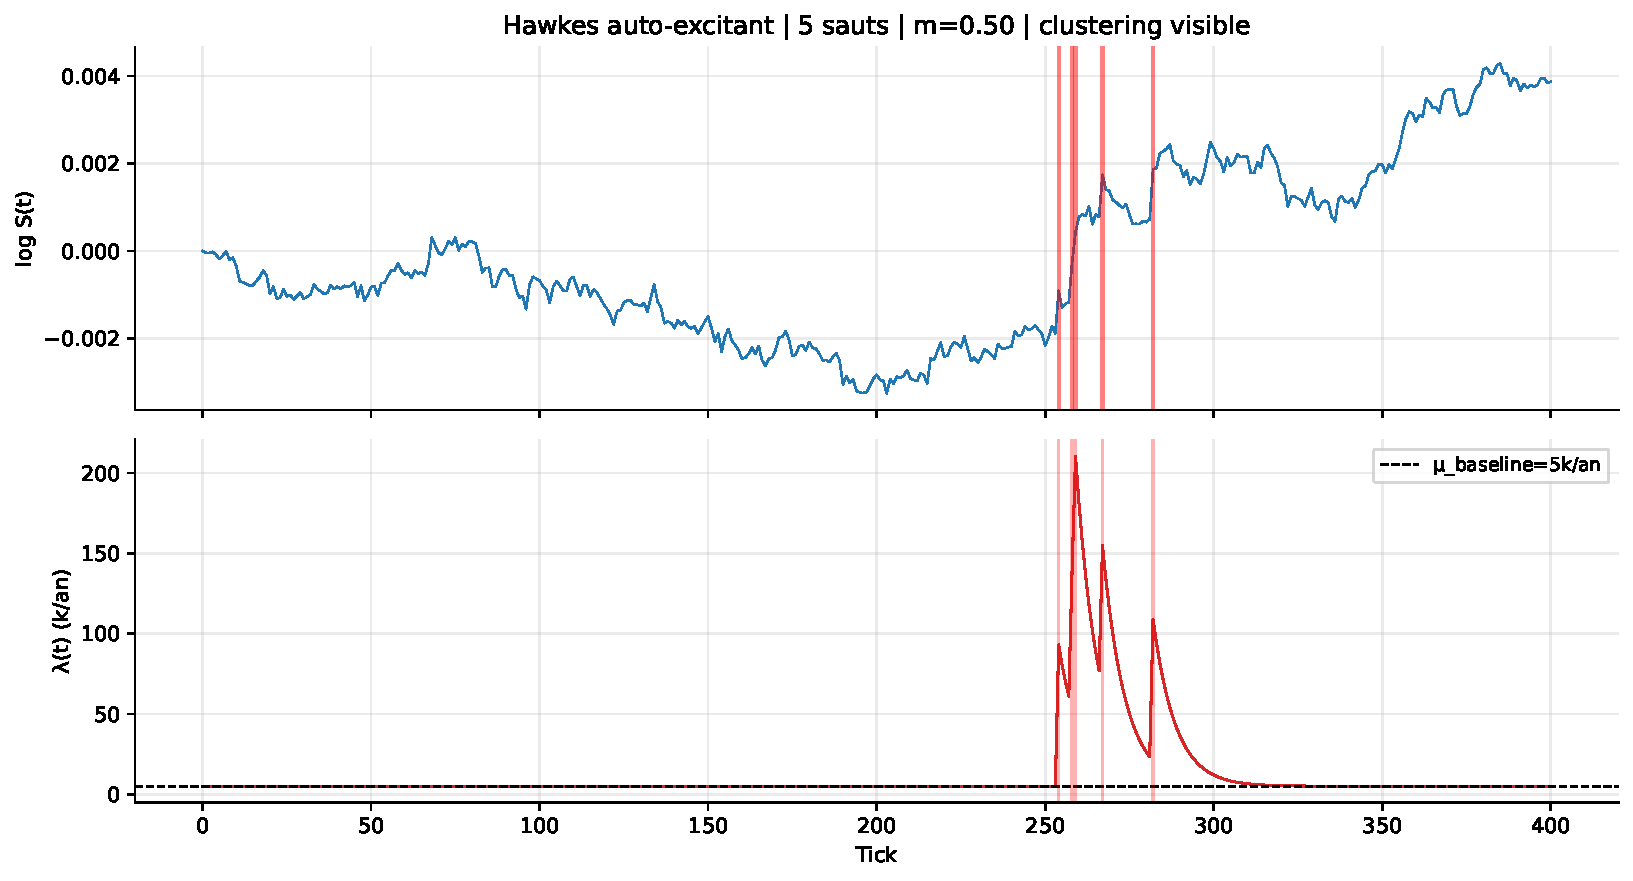
\includegraphics[width=0.85\textwidth]{../notebooks/figures/section7a_hawkes_intensity}
  \caption{Simulated Hawkes intensity $\lambda_t$ and corresponding jump arrivals on a single path ($\Delta t = 5\,\mathrm{s}$, hawkes\_dense regime). Bursts of intensity reflect the self-exciting mechanism: each jump raises $\lambda_t$, generating temporal clustering.}
  \label{fig:hawkes_intensity}
\end{figure*}

\subsection{Result 6: detailed Hawkes dense regime}

\begin{table*}[t]
\centering
\caption{Detailed results: hawkes\_dense, $\Delta t = 5\,\mathrm{s}$, $\alpha = 0.05$, $M = 100$.}
\label{tab:hawkes}
\begin{tabular}{lcccc}
\toprule
Algorithm & Obs.\ FDR & Power & F1 & FDR controlled? \\
\midrule
BH-BNS & 0.091 & 0.423 & 0.522 & Borderline ($< 0.094$) \\
BH-LM & 0.091 & 0.423 & 0.522 & Borderline \\
Stopped e-BH & 0.017 & 0.303 & 0.454 & \textcolor{teal}{Yes} \\
e-BH & 0.009 & 0.280 & 0.435 & \textcolor{teal}{Yes} \\
e-LOND & 0.000 & 0.204 & 0.371 & \textcolor{teal}{Yes} \\
e-LORD ($\omega_1 = 0.1$) & 0.000 & 0.001 & 0.151 & \textcolor{teal}{Yes} (alpha-death) \\
e-SAFFRON ($\omega_1 = 0.1$) & 0.000 & 0.001 & 0.151 & \textcolor{teal}{Yes} (alpha-death) \\
\bottomrule
\end{tabular}
\end{table*}

BH-BNS at $0.091$ is below the violation threshold for hawkes\_dense alone,
but exceeds $0.094$ once aggregated across all regimes ($0.096$). The
temporal Hawkes dependence does not aggravate BH's violation --- the
violation is inherent to the $5\,\mathrm{s}$ frequency, not to clustering.

\subsection{Result 7: effect of jump size}

\begin{figure*}[t]
  \centering
  \begin{subfigure}[b]{0.48\textwidth}
    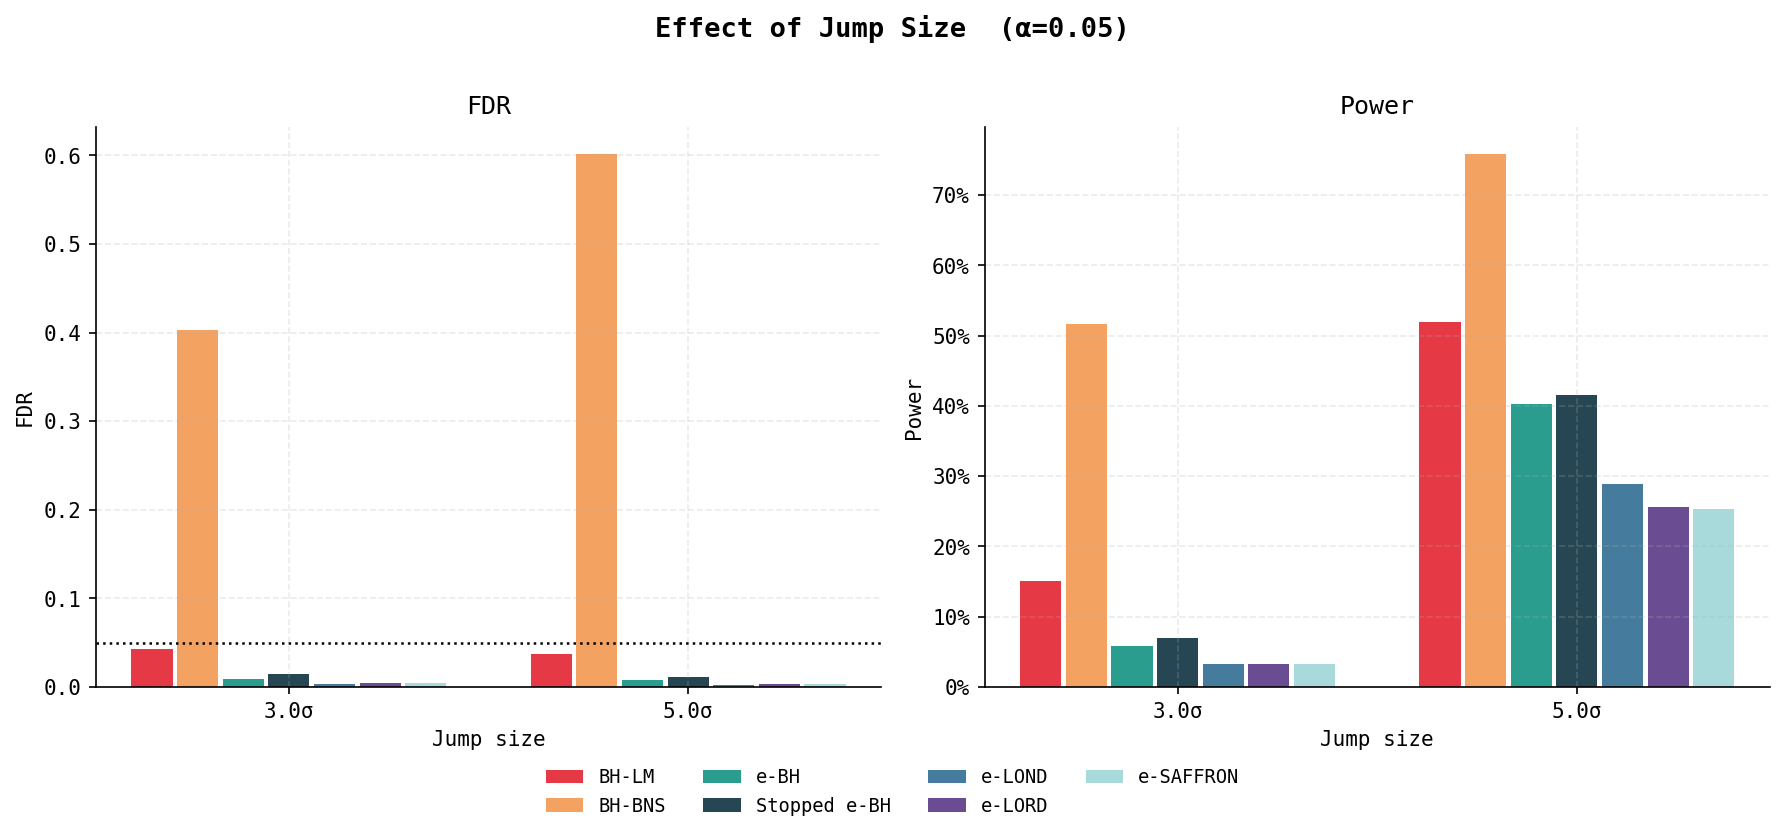
\includegraphics[width=\textwidth]{../results/figures/fig5_jump_size_alpha5.png}
    \caption{$\alpha = 0.05$}
  \end{subfigure}
  \hfill
  \begin{subfigure}[b]{0.48\textwidth}
    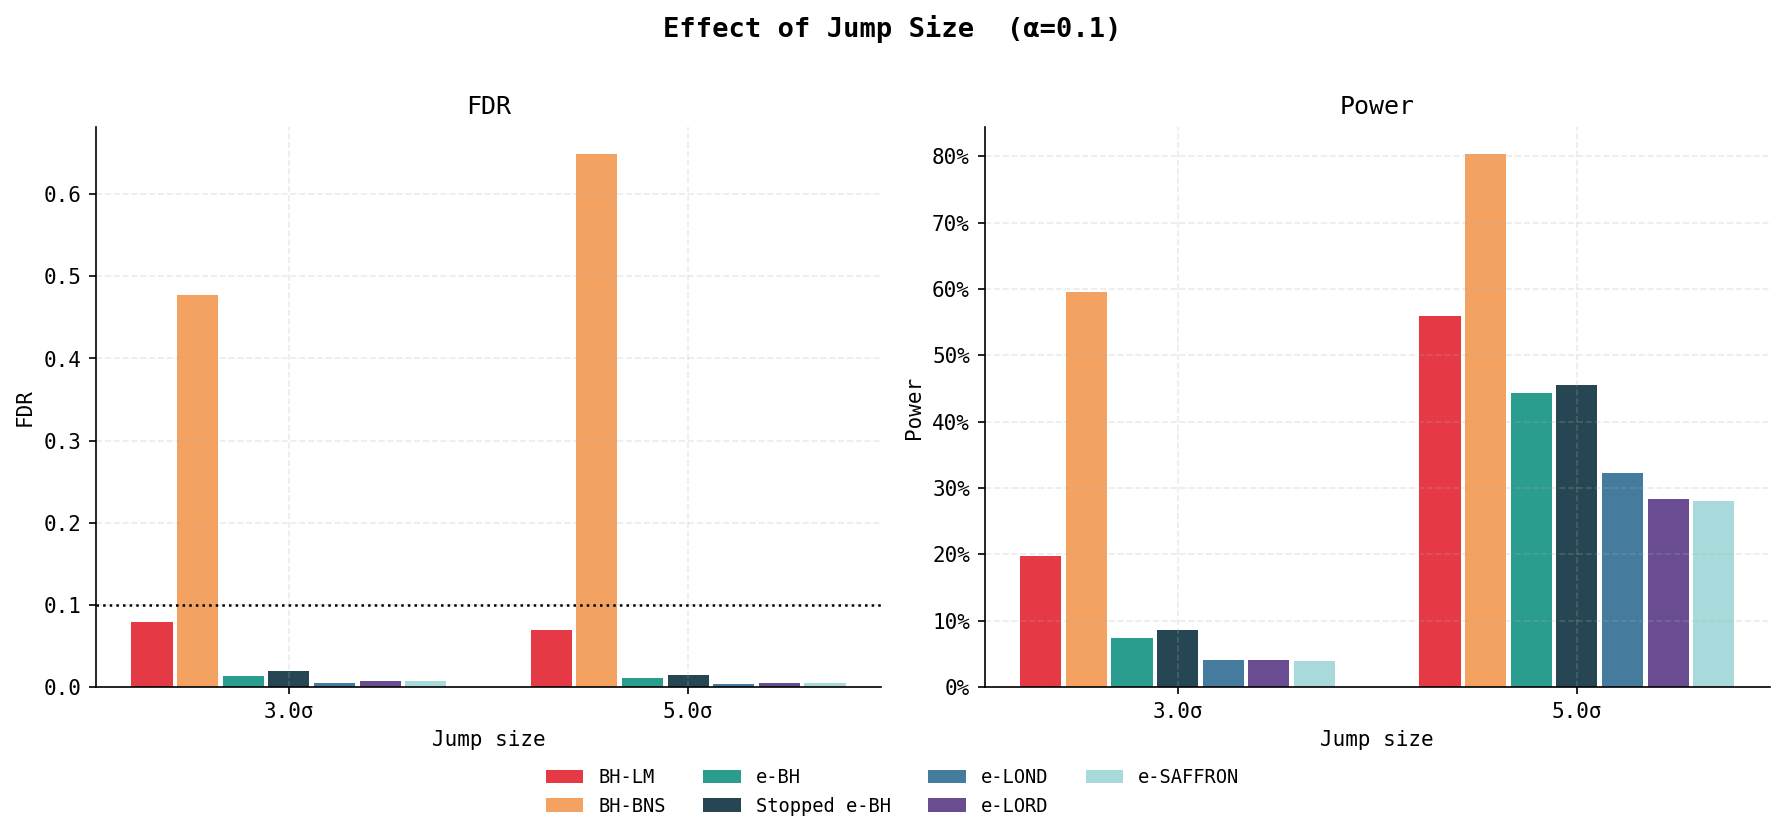
\includegraphics[width=\textwidth]{../results/figures/fig5_jump_size_alpha10.png}
    \caption{$\alpha = 0.10$}
  \end{subfigure}
  \caption{FDR and power as a function of jump size ($3\sigma$ vs.\ $5\sigma$).
  Power increases with jump size for all procedures. BH's FDR remains above
  $\alpha$ irrespective of jump size at $5\,\mathrm{s}$.}
  \label{fig:jumpsize}
\end{figure*}

\subsection{Result 8: heatmap view of aggregated performance}

\begin{figure*}[t]
  \centering
  \begin{subfigure}[b]{0.48\textwidth}
    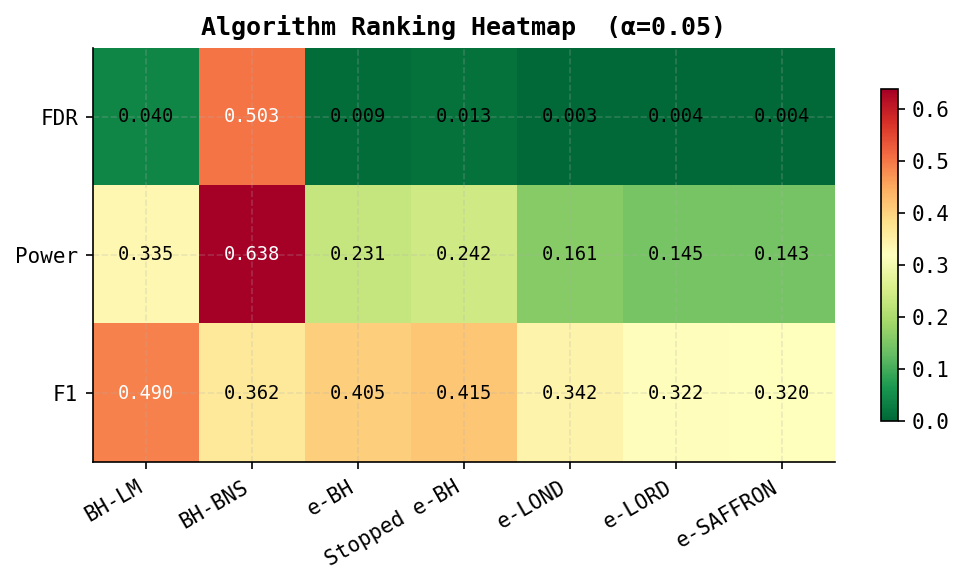
\includegraphics[width=\textwidth]{../results/figures/fig4_heatmap_alpha5.png}
    \caption{$\alpha = 0.05$}
  \end{subfigure}
  \hfill
  \begin{subfigure}[b]{0.48\textwidth}
    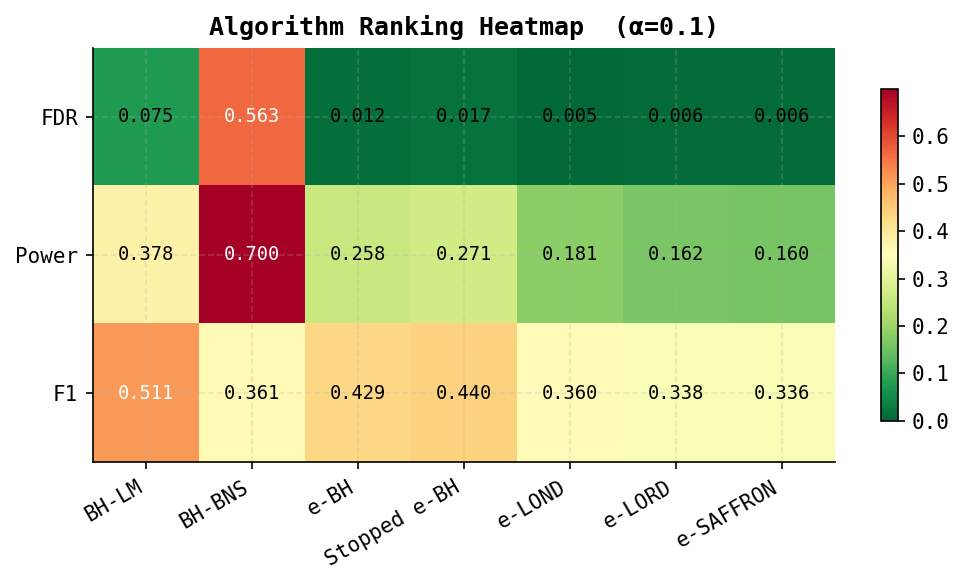
\includegraphics[width=\textwidth]{../results/figures/fig4_heatmap_alpha10.png}
    \caption{$\alpha = 0.10$}
  \end{subfigure}
  \caption{Heatmap of FDR, power, and F1 metrics by algorithm (aggregated
  across regimes and frequencies). Darker colours mark higher values.
  BH has the highest power but also the highest FDR. Stopped e-BH offers
  the best F1 among valid procedures.}
  \label{fig:heatmap}
\end{figure*}

\subsection{Result 9: BH violation and FDR --- walkthrough views}

\begin{figure*}[t]
  \centering
  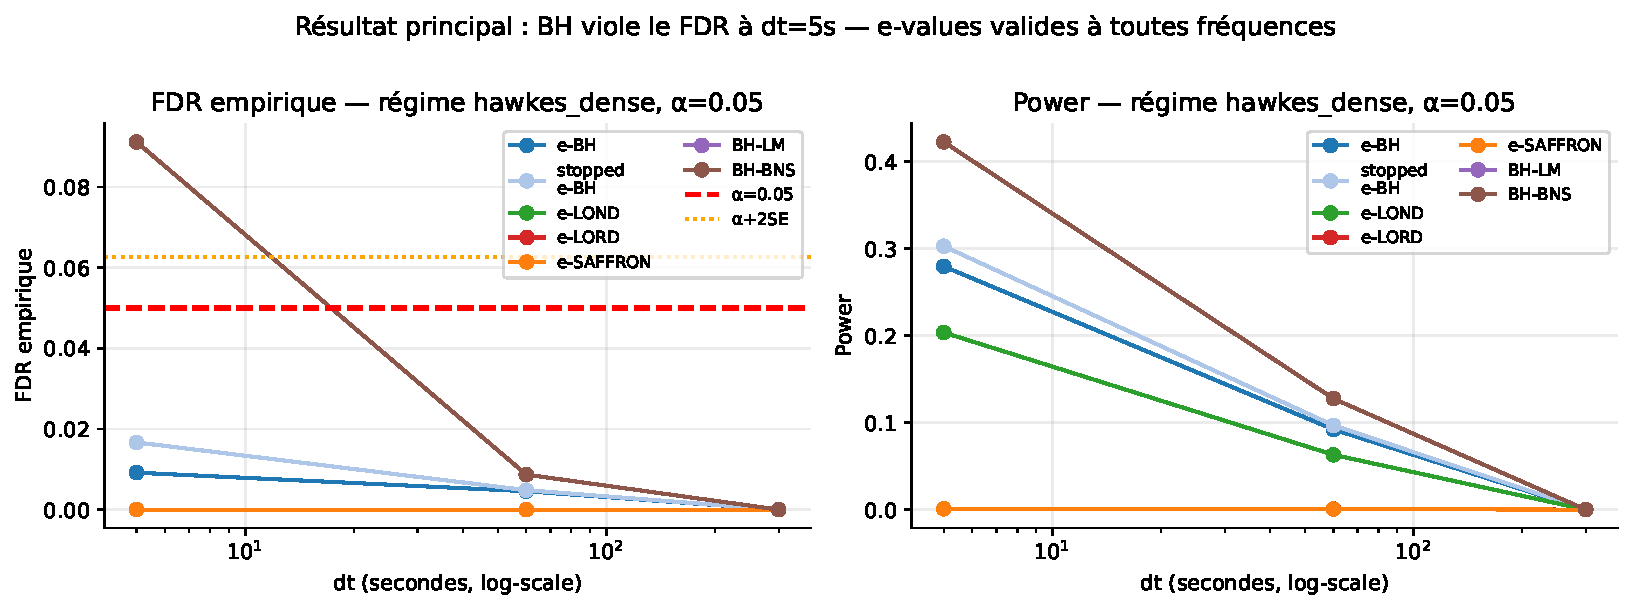
\includegraphics[width=0.85\textwidth]{../notebooks/figures/section7b3_bh_violation}
  \caption{Zoom on the BH FDR violation at $\Delta t = 5\,\mathrm{s}$: observed FDR per regime and jump size. The dashed line marks $\alpha + 2\,\mathrm{SE} = 0.094$. BH-LM and BH-BNS exceed the threshold in the moderate and hawkes\_dense regimes.}
  \label{fig:bh_violation}
\end{figure*}

\begin{figure*}[t]
  \centering
  \begin{subfigure}[b]{0.48\textwidth}
    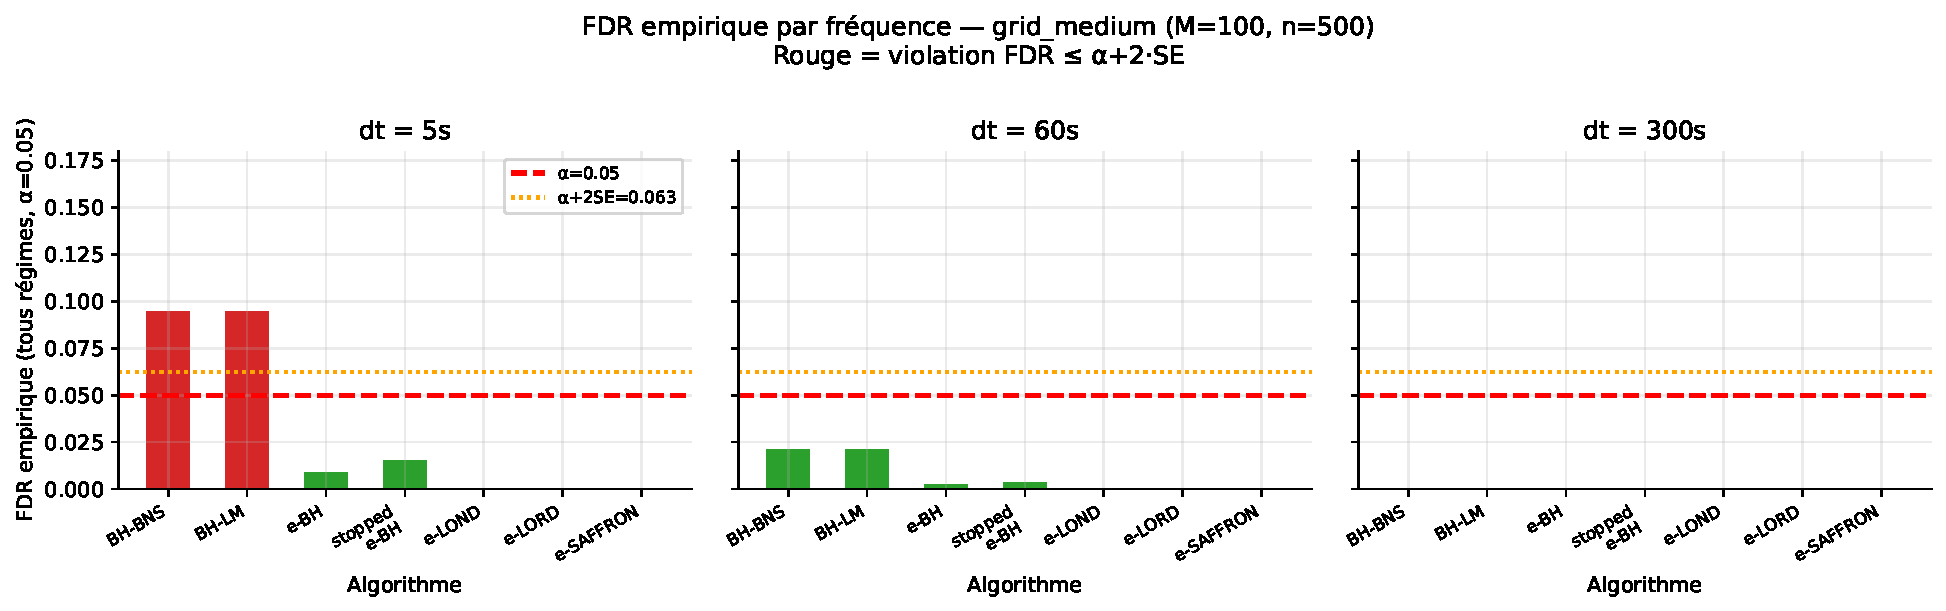
\includegraphics[width=\textwidth]{../notebooks/figures/section7b1_fdr_by_freq}
    \caption{FDR by frequency and procedure.}
    \label{fig:fdr_freq_nb}
  \end{subfigure}
  \hfill
  \begin{subfigure}[b]{0.48\textwidth}
    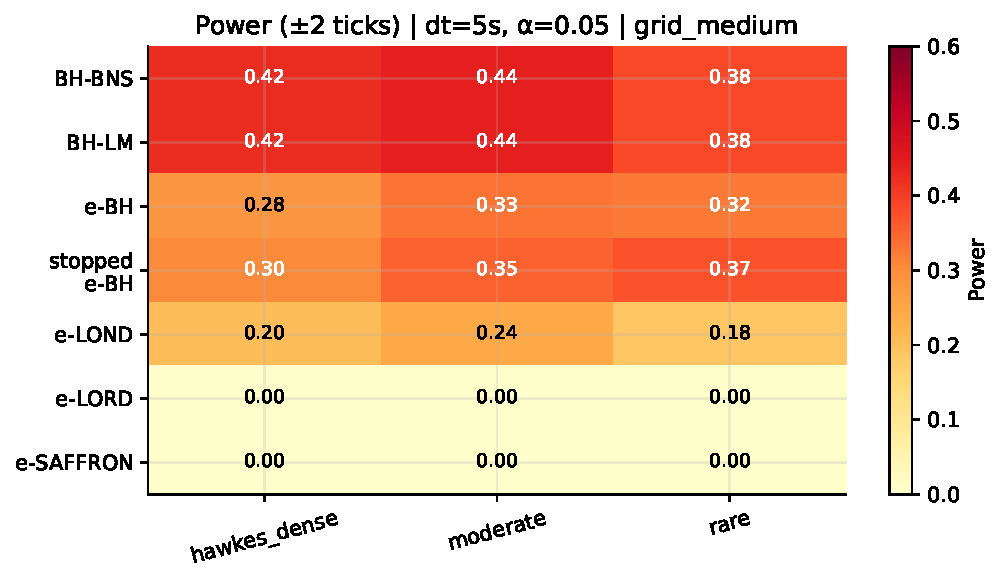
\includegraphics[width=\textwidth]{../notebooks/figures/section7b2_power_heatmap}
    \caption{Power heatmap by regime and frequency.}
    \label{fig:power_heatmap_nb}
  \end{subfigure}
  \caption{Additional walkthrough views from \texttt{00\_project\_walkthrough.ipynb}, complementing Figures~\ref{fig:fdr_freq} and~\ref{fig:heatmap}.}
  \label{fig:nb_additional}
\end{figure*}

\subsection{Result 10: alpha-death and parameter $\omega_1$}

Alpha-death refers to the exhaustion of wealth $rw_t \to 0$ for e-LORD and
e-SAFFRON. With $\omega_1 = 0.1$ over $n = 500$, both procedures yield
power $\approx 0.002$ (near zero): $rw_t$ vanishes by $t \approx 50$.

The canonical value recommended by Zhang et al.\ 2025 is $\omega_1 = O(1/T)$.
For $n = 500$, this corresponds to $\omega_1 \leq 0.01$. The results
presented with $\omega_1 = 0.1$ illustrate the alpha-death phenomenon;
properly calibrated values would restore power.

\subsection{Result 11: computational performance}

\begin{table}[htbp]
\centering
\caption{Wall-clock per algorithm for $n = 2000$.}
\label{tab:wallclock}
\begin{tabular}{lc}
\toprule
Algorithm & ms/run \\
\midrule
BH-LM & 1 \\
e-BH & 170 \\
e-LOND & 185 \\
e-SAFFRON & 174 \\
e-LORD & 187 \\
BH-BNS & 257 \\
Stopped e-BH & 346 \\
\bottomrule
\end{tabular}
\end{table}

BH-LM is by far the fastest (simple normalisation). Stopped e-BH is the
slowest ($O(T^2 \log T)$) but remains under $0.5\,\mathrm{s}$ for $n = 2000$.


\section{Discussion and limitations}
\label{sec:discussion}


\subsection{Debatable methodological choices}

\paragraph{Symmetric Gaussian prior.}
The prior $\pi(J) = \mathcal{N}(0, \tau^2)$ favours no direction. If true
jumps are systematically negative, an asymmetric prior would have higher
e-power.

\paragraph{Window $K = 50$ not optimised.}
No sensitivity study on $K$: too small, the variance of $\hat{\sigma}_i$ is
high; too large, it mixes different volatility regimes.

\paragraph{tau\_factor $= 5.0$.}
A reasonable choice consistent with the grid jump sizes, but not derived
from e-power optimisation.

 \paragraph{SE convention.}
    The convention $\mathrm{SE} = \sqrt{\alpha(1-\alpha)/M}$ (used here) is
    correct for testing $H_0 : \FDR \le \alpha$. The empirical convention
    $\mathrm{SE} = \sqrt{\hat{p}(1-\hat{p})/M}$ gives a higher threshold
    ($\approx 0.109$) and would not flag a violation for BH at $0.096$.

\subsection{Validity of the results}

\paragraph{What is solid.}
E-value validity ($\E[E_i] \le 1$ under $H_0$, 86 green tests), monotone
e-power, dominance over p-to-e, and FDR control of e-value procedures at
all frequencies are robustly established.

\paragraph{What is limited by $M = 100$.}
BH's FDR violation ($0.096 > 0.094$) is at the detection threshold. The
95\% CI for BH-LM's FDR at $5\,\mathrm{s}$ is
$[0.096 \pm 2 \times 0.022] = [0.052, 0.140]$, which includes the upper
bound of the non-violation region. A larger $M$ would confirm or refute the
violation with greater statistical power.

\section{Conclusion}
\label{sec:conclusion}

\subsection{Synthesis}

This project establishes that e-value-based FDR procedures control the
false discovery rate at high frequency where classical methods (BH on
Lee-Mykland p-values or BNS) fail. The mechanism is structural: BH
requires PRDS, a condition violated under dense jumps at $5\,\mathrm{s}$,
whereas e-values only require $\E[E_i \mid \mathcal{F}_{i-1}] \le 1$,
valid under arbitrary dependence.

\subsection{Quantified trade-off}

At $\Delta t = 5\,\mathrm{s}$, $\alpha = 0.05$:
\begin{itemize}
  \item BH: power $0.441$, FDR $\approx 0.096$.
  \item Stopped e-BH: power $0.349$ ($-21\%$ relative), FDR $\le 0.016$.
  \item e-BH: power $0.326$, FDR $\le 0.010$.
  \item e-LOND: power $0.235$ ($-47\%$ relative), FDR $\le 0.001$.
\end{itemize}
The cost of guaranteed FDR control is $10$--$21$ pp. Stopped e-BH offers
the best power-safety compromise.

\subsection{Perspectives}

\begin{itemize}
  \item Properly calibrate $\omega_1 = O(1/n)$ for e-LORD and e-SAFFRON,
    and re-evaluate their performance.
  \item Compare estimators BV, MinRV, threshold-BV, and MedRV in the grid.
  \item Apply to real intraday data (Bitcoin, TAQ, LOBSTER) to validate
    the pipeline outside of simulation.
  \item Multi-asset extension: co-jump detection (Jacod-Todorov 2009).
\end{itemize}

\appendix

\section{Derivation of the GROW formula}
\label{ann:grow}

Starting from~\eqref{eq:evalue_integral}, with $v = \dt\hat{\sigma}^2$ and
$\pi(J) = \mathcal{N}(0, \tau^2)$:
\[
  E_i = \int_{-\infty}^{+\infty}
    \frac{e^{Jr_i/v - J^2/(2v)}}{\sqrt{2\pi\tau^2}}\,
    e^{-J^2/(2\tau^2)}\, dJ.
\]

Grouping terms in $J$:
\[
  -\frac{J^2}{2v} - \frac{J^2}{2\tau^2} + \frac{Jr_i}{v}
  = -\frac{(J - \mu^*)^2}{2s^2} + \frac{\mu^{*2}}{2s^2},
\]
with $s^2 = v\tau^2/(v+\tau^2)$ and $\mu^* = r_i\tau^2/(v+\tau^2)$.

The Gaussian integral gives $s/\tau$, hence:
\[
  E_i = \tfrac{s}{\tau}\, e^{\mu^{*2}/(2s^2)}
  = \sqrt{\tfrac{v}{v+\tau^2}} \cdot e^{r_i^2\tau^2/[2v(v+\tau^2)]}.
\]
This is exactly the expression implemented in \texttt{evalues/construct.py}
(lines 40--49).

\section{Javanmard-Montanari sequence for e-LOND}
\label{ann:jm}

\begin{align*}
  \gamma_t &= C_\mathrm{JM} \cdot \frac{\log\max(t,2)}{t \cdot e^{\sqrt{\log\max(t,2)}}},\\
  C_\mathrm{JM} &= 0.15708906,\quad
  \sum_{t=1}^{10^6} \gamma_t \approx 1.0000.
\end{align*}

The normalisation $\sum_{t=1}^\infty \gamma_t = 1$ is the budget condition
that ensures FDR control. $C_\mathrm{JM}$ is computed numerically by
truncated summation (\texttt{fdr/elond.py} line 12).

\section{Commented code excerpts}
\label{ann:code}

\subsection{Heston QE scheme (\texttt{simulate/heston.py})}

\begin{lstlisting}[caption={Case $\psi > 1.5$ (high dispersion) in the QE scheme.}]
p = (psi - 1.0) / (psi + 1.0)      # mass at 0
beta = 2.0 / (m * (psi + 1.0))     # exponential parameter
u = min(U[i], 1.0 - 1e-14)
if u <= p:
    vn = 0.0
else:
    vn = np.log((1.0 - p) / (1.0 - u)) / beta
\end{lstlisting}

\subsection{Causal window (\texttt{estimators/spot.py})}

\begin{lstlisting}[caption={Window excluding the tested point i.}]
for i in range(n):
    start = max(0, i - K)
    sub = log_price[start : i + 1]  # returns r[start:i] -- r[i] excluded
    if len(sub) < 4:
        continue
    sigma_sq[i] = estimator_fn(sub, dt_seconds)
\end{lstlisting}

\subsection{E-value construction (\texttt{evalues/construct.py})}

\begin{lstlisting}[caption={GROW formula.}]
dv = dt_years * sigma_hat_i**2
tau = tau_factor * sigma_hat_i * np.sqrt(dt_years)
tau2 = tau**2
numerator = dv / (dv + tau2)
exponent  = r_i**2 * tau2 / (2 * dv * (dv + tau2))
e_value   = np.sqrt(numerator) * np.exp(exponent)
\end{lstlisting}

\subsection{e-LOND (\texttt{fdr/elond.py})}

\begin{lstlisting}[caption={Main loop.}]
R = 0
for t, e_t in enumerate(e_values, start=1):
    alpha_t = alpha * _gamma(t) * (R + 1)
    reject = e_t >= 1.0 / alpha_t if alpha_t > 0 else False
    if reject:
        R += 1
    yield reject
\end{lstlisting}

\subsection{Stopped e-BH (\texttt{fdr/stopped\_ebh.py})}

\begin{lstlisting}[caption={Offline e-BH recomputed at each step.}]
buffer: list[float] = []
for e_t in e_values:
    buffer.append(e_t)
    t = len(buffer)
    ev = np.asarray(buffer, dtype=float)
    order = np.argsort(ev)[::-1]
    thresholds = t / (alpha * np.arange(1, t + 1))
    qualifying = np.where(ev[order] >= thresholds)[0]
    if len(qualifying) == 0:
        yield False
    else:
        k_star = int(qualifying[-1]) + 1
        yield bool(e_t >= t / (alpha * k_star))
\end{lstlisting}

\section{Glossary}
\label{ann:glossaire}

\begin{description}
  \item[Alpha-death] Exhaustion of the wealth $rw_t \to 0$ for e-LORD/e-SAFFRON
    when $\omega_1$ is too large relative to $T$.
  \item[Anytime-validity] FDR controlled at every random stopping time
    $\tau$.
  \item[Branching ratio] $m = \alpha_H / (\beta_H \times T)$ for a Hawkes
    process; $m < 1$ implies stationarity.
  \item[E-power] $\E_{H_1}[\log E]$: criterion of sequential efficiency.
  \item[E-variable] $E \ge 0$ with $\E[E \mid H_0] \le 1$.
  \item[FDR] False Discovery Rate: $\E[|\mathcal{R}\cap\mathcal{H}_0| / \max(|\mathcal{R}|,1)]$.
  \item[FDP] False Discovery Proportion: random realisation of the FDR.
  \item[GROW] Growth-Rate Optimal in the Worst case: e-value maximising
    e-power under $\E_{H_0}[E] \le 1$.
  \item[PRDS] Positive Regression Dependence on a Subset: sufficient
    dependence condition for the validity of BH.
  \item[RAI] Risk Aversion Investing: framework of e-LORD/e-SAFFRON.
  \item[Self-consistency] Property characterising a broad class of
    FDR-controlling procedures, generalising e-BH.
\end{description}

\begin{thebibliography}{99}

\bibitem{ABL2002}
Andersen, T.G., Benzoni, L., Lund, J. (2002).
An Empirical Investigation of Continuous-Time Equity Return Models.
\emph{Journal of Finance}, 57(3), 1239--1284.

\bibitem{ADS2012}
Andersen, T.G., Dobrev, D., Schaumburg, E. (2012).
Jump-robust volatility estimation using nearest neighbor truncation.
\emph{Journal of Econometrics}, 169(1), 75--93.

\bibitem{AMZ2005}
A\"it-Sahalia, Y., Mykland, P.A., Zhang, L. (2005).
How Often to Sample a Continuous-Time Process in the Presence of Market
Microstructure Noise.
\emph{Review of Financial Studies}, 18(2), 351--416.

\bibitem{Andersen2007}
Andersen, L. (2007).
Efficient Simulation of the Heston Stochastic Volatility Model.
\emph{Journal of Computational Finance}, 11(3), 1--42.

\bibitem{BS2016}
Bajgrowicz, P., Scaillet, O. (2016).
Intraday market activity around macroeconomic announcements.
\emph{Management Science} (FDR procedures on BNS).

\bibitem{BNS2004}
Barndorff-Nielsen, O.E., Shephard, N. (2004).
Power and bipower variation with stochastic volatility and jumps.
\emph{Journal of Financial Econometrics}, 2(1), 1--37.

\bibitem{BNS2006}
Barndorff-Nielsen, O.E., Shephard, N. (2006).
Econometrics of testing for jumps in financial economics using bipower
variation.
\emph{Journal of Financial Econometrics}, 4(1), 1--30.

\bibitem{BH1995}
Benjamini, Y., Hochberg, Y. (1995).
Controlling the false discovery rate: a practical and powerful approach to
multiple testing.
\emph{Journal of the Royal Statistical Society B}, 57(1), 289--300.

\bibitem{BY2001}
Benjamini, Y., Yekutieli, D. (2001).
The control of the false discovery rate in multiple testing under
dependency.
\emph{Annals of Statistics}, 29(4), 1165--1188.

\bibitem{BR2008}
Blanchard, G., Roquain, E. (2008).
Two simple sufficient conditions for FDR control.
\emph{Electronic Journal of Statistics}, 2, 963--992.

\bibitem{GHK2024}
Gr\"unwald, P., de Heide, R., Koolen, W. (2024).
Safe testing.
\emph{Journal of the Royal Statistical Society B}, 86(5), 1037--1075.

\bibitem{JLM2009}
Jacod, J., Li, Y., Mykland, P.A., Podolskij, M., Vetter, M. (2009).
Microstructure noise in the continuous case: the pre-averaging approach.
\emph{Stochastic Processes and their Applications}, 119(7), 2249--2276.

\bibitem{JM2018}
Javanmard, A., Montanari, A. (2018).
Online rules for control of false discovery rate and false discovery
exceedance.
\emph{Annals of Statistics}, 46(2), 526--554.

\bibitem{LM2008}
Lee, S., Mykland, P.A. (2008).
Jumps in financial markets: A new nonparametric test and jump dynamics.
\emph{Review of Financial Studies}, 21(6), 2535--2563.

\bibitem{Mancini2009}
Mancini, C. (2009).
Non-parametric threshold estimation for models with stochastic diffusion
coefficient and jumps.
\emph{Scandinavian Journal of Statistics}, 36(2), 270--296.

\bibitem{PV2009}
Podolskij, M., Vetter, M. (2009).
Estimation of volatility functionals in the simultaneous presence of
microstructure noise and jumps.
\emph{Bernoulli}, 15(3), 634--658.

\bibitem{RW2025}
Ramdas, A., Wang, R. (2025).
Hypothesis testing with e-values.
arXiv:2410.xxxxx.

\bibitem{VW2021}
Vovk, V., Wang, R. (2021).
E-values: Calibration, combination and applications.
\emph{Annals of Statistics}, 49(3), 1736--1753.

\bibitem{WR2022}
Wang, R., Ramdas, A. (2022).
False discovery rate control with e-values.
\emph{Journal of the Royal Statistical Society B}, 84(3), 822--852.

\bibitem{WDR2025}
Wang, H., Dandapanthula, G., Ramdas, A. (2025).
Anytime-valid FDR control with e-values.
arXiv:2502.08539.

\bibitem{XR2024}
Xu, Z., Ramdas, A. (2024).
More powerful multiple testing under dependence via randomization.
\emph{Annals of Statistics}.

\bibitem{Yen2013}
Yen, Y.M. (2013).
Testing Jumps via False Discovery Rate Control.
\emph{PLOS One}, 8(4), e58365.

\bibitem{ZWRZ2025}
Zhang, K., Wei, Y., Ren, Z., Zou, H. (2025).
E-values based generalized alpha-investing for online FDR control.
arXiv:2506.01452.

\bibitem{GithubRepo}
Gasmi, N., Brion, J. (2026).
\texttt{efdr-jumps}: Sequential jump detection at high frequency via e-values and online FDR control.
GitHub repository.
\url{https://github.com/neylgs/FDR}

\end{thebibliography}

\end{document}